\documentclass[11pt]{article}

\usepackage{iftex}
\ifPDFTeX
  \usepackage[utf8]{inputenc}
\else
  \usepackage{fontspec}
  \usepackage{xeCJK}
  \setmainfont{Times New Roman}
  \setsansfont{Helvetica}
  \setmonofont{Noto Sans Mono CJK KR}
  \setCJKmainfont{Apple SD Gothic Neo}
  \setCJKsansfont{Apple SD Gothic Neo}
  \setCJKmonofont{Noto Sans Mono CJK KR}
\fi
\usepackage[a4paper,margin=1in]{geometry}
\usepackage{amsmath}
\usepackage{amssymb}
\usepackage{booktabs}
\usepackage{tabularx}
\usepackage{longtable}
\usepackage{array}
\usepackage{xcolor}
\usepackage{hyperref}
\usepackage{enumitem}
\usepackage{fancyhdr}
\usepackage{microtype}
\usepackage{listings}
\usepackage{graphicx}
\usepackage{tikz}
\usepackage[most]{tcolorbox}
\usetikzlibrary{arrows.meta,positioning,shapes.geometric,fit,backgrounds}
\graphicspath{{output/latex/figures/}{figures/}}

\hypersetup{
  colorlinks=true,
  linkcolor=black,
  citecolor=black,
  urlcolor=blue
}

\pagestyle{fancy}
\fancyhf{}
\lhead{Physical AI Risk Taxonomy Technical Report}
\rhead{}
\lfoot{}
\cfoot{\thepage}
\rfoot{}
\setlength{\headheight}{14pt}
\setlength{\parskip}{0.55em}
\setlength{\parindent}{0pt}
\renewcommand{\arraystretch}{1.16}

\definecolor{sqlkeyword}{RGB}{0,76,151}
\definecolor{sqlcomment}{RGB}{0,122,74}
\definecolor{sqlstring}{RGB}{154,54,42}
\definecolor{sqlbackground}{RGB}{248,250,252}
\definecolor{sqlrule}{RGB}{198,207,217}
\definecolor{flowblue}{RGB}{31,93,165}
\definecolor{flowgreen}{RGB}{31,132,87}
\definecolor{floworange}{RGB}{191,111,38}
\definecolor{flowpurple}{RGB}{104,72,166}
\definecolor{flowgray}{RGB}{87,96,111}
\definecolor{flowg1}{gray}{0.45}
\definecolor{flowg2}{gray}{0.30}
\definecolor{flowg3}{gray}{0.60}
\definecolor{flowg4}{gray}{0.38}
\definecolor{flowg5}{gray}{0.72}
\definecolor{reportblue}{RGB}{23,52,88}

\lstdefinestyle{patstatsql}{
  language=SQL,
  basicstyle=\ttfamily\scriptsize,
  keywordstyle=\color{sqlkeyword}\bfseries,
  commentstyle=\color{sqlcomment}\itshape,
  stringstyle=\color{sqlstring},
  numbers=left,
  numberstyle=\tiny\color{gray},
  stepnumber=1,
  numbersep=6pt,
  breaklines=true,
  breakatwhitespace=false,
  columns=fullflexible,
  keepspaces=true,
  showstringspaces=false,
  frame=single,
  rulecolor=\color{sqlrule},
  backgroundcolor=\color{sqlbackground},
  captionpos=b
}

\lstdefinestyle{wosquery}{
  basicstyle=\ttfamily\scriptsize,
  keywordstyle=\color{sqlkeyword}\bfseries,
  stringstyle=\color{sqlstring},
  morekeywords={TS,CU,PY,DT,AND,OR},
  alsoletter={=},
  numbers=left,
  numberstyle=\tiny\color{gray},
  stepnumber=1,
  numbersep=6pt,
  breaklines=true,
  breakatwhitespace=false,
  columns=fullflexible,
  keepspaces=true,
  showstringspaces=false,
  frame=single,
  rulecolor=\color{sqlrule},
  backgroundcolor=\color{sqlbackground},
  captionpos=b
}

\newcommand{\DPAI}{\mathcal{D}_{\mathrm{PAI}}}
\newcommand{\Enc}{\mathrm{Enc}_{\theta}}
\newcommand{\simcos}{\mathrm{sim}_{\cos}}
\newcommand{\Harm}{\operatorname{Harm}}

% Figure/table note rendered as a full-width justified block (not centered)
\newcommand{\fignote}[1]{\par\vspace{0.25em}\noindent\begin{minipage}{\linewidth}\footnotesize\textit{Note:} #1\end{minipage}}

\newtcolorbox{algobox}[1]{
  enhanced,
  breakable,
  colback=black!2,
  colframe=black!68,
  boxrule=0.65pt,
  arc=1.5pt,
  left=7pt,
  right=7pt,
  top=6pt,
  bottom=6pt,
  fonttitle=\bfseries,
  title={#1}
}

\begin{document}

\begin{titlepage}
\thispagestyle{empty}
\vspace*{0.6in}
{\sffamily\bfseries\Large Technical Report\par}
\vspace{0.10in}
{\sffamily\bfseries\Large\color{red}DRAFT --- for review, not for citation\par}
\vspace{0.16in}
{\color{reportblue}\rule{\linewidth}{1.2pt}\par}
\vspace{0.28in}
{\sffamily\bfseries\Huge A Hybrid Corpus-to-Taxonomy Pipeline for Physical AI Risk Cards\par}
\vspace{0.16in}
{\sffamily\Large Data Collection, Processing, Deduplication, and\ Hierarchical Assignment\par}
\vspace{0.28in}
{\color{reportblue}\rule{\linewidth}{0.7pt}\par}
\vspace{0.5in}

\begin{tabularx}{\linewidth}{>{\bfseries}p{0.27\linewidth}X}
Report type & Technical Report \\
Report title & A Hybrid Corpus-to-Taxonomy Pipeline for Physical AI Risk Cards \\
Report version & v1.0 --- \textbf{Draft (for review)} \\
Taxonomy release & Responsible AI Risk Taxonomy v2.0, Physical AI Risk Taxonomy slice \\
Author & Youngsam Chun \\
Affiliation & Responsible AI Dept., Frontier AI Lab \\
Contact & \href{mailto:ys.chun@kt.com}{ys.chun@kt.com} \\
Local data snapshot & Verified on 2026-07-04 \\
Primary artifacts & HTML taxonomy, CSV/JSON card exports, reference map, methodology PDF \\
Reproducibility status & Local source queries, file-level denominators, algorithms, and release checks documented \\
\end{tabularx}

\vfill
{\sffamily Responsible AI Dept., Frontier AI Lab\par}
{\sffamily July 2026\par}
\end{titlepage}

\section*{Executive Summary}
\addcontentsline{toc}{section}{Executive Summary}
This manuscript documents the data collection, processing, analysis, and risk-card generation procedure used to construct the Physical AI slice of the Responsible AI Risk Taxonomy v2.0. The workflow follows a hybrid taxonomy design: high-level structure is anchored in authoritative safety, risk-management, and embodied-AI references, while L4 risk cards are generated bottom-up from a multi-source corpus of scientific publications, policy reports, and patents. The updated local integrated document space contains 3,906,767 AI records, 741,428 AI infrastructure records, 383,149 Physical AI records, and 82,971 Physical AI risk records after within-group deduplication across scientific publications, policy reports, and patents. The released local taxonomy snapshot contains 182 L4 risk cards, 24 L3 sub-categories, 3 L2 categories, and 360 card-level evidence/reference rows. We formalize two procedures: (i) risk-candidate generation with semantic deduplication and (ii) EM-based L3 family assignment.

\textbf{Keywords:} Physical AI; AI risk taxonomy; robotics safety; embodied AI; cyber-physical systems; semantic deduplication; BGE-M3; HDBSCAN; reproducible technical report.

\textbf{Reproducibility statement.} This report is written as a technical reconstruction protocol. It specifies the source families, retrieval artifacts, local file denominators, filtering thresholds, embedding inputs, clustering and deduplication procedures, hierarchy assignment procedure, validation checks, and release artifacts required to reproduce the Physical AI Risk Taxonomy construction workflow.

\tableofcontents
\newpage

\section{Scope and Design Rationale}

Physical AI is defined here as AI deployed in systems that sense, reason, and act in the physical world, including robots, humanoids, drones, autonomous vehicles, cyber-physical systems, and embodied agents. This scope follows recent Physical AI and embodied-safety work that treats world models, robot constitutions, and embodied benchmarks as distinct from text-only AI risk settings~\cite{nvidia-cosmos,sermanet-asimov,asimov2}. The taxonomy is organized as:
\begin{equation}
\begin{aligned}
L0~\text{Ownership Levels} &\rightarrow L1~\text{Physical AI Risks} \\
&\rightarrow L2~\text{Categories} \rightarrow L3~\text{Sub-categories} \rightarrow L4~\text{Risk Cards}.
\end{aligned}
\end{equation}
The L2 layer distinguishes the locus of risk responsibility: internal system safety, interaction safety at the human/environment interface, and broader societal safety. The L4 layer is the operational unit: each card has a stable identifier, bilingual label and definition, severity and probability proxies, short evidence justifications, references, and 3H1R alignment tags.

The methodological problem is that Physical AI risk taxonomies cannot be built purely top-down or purely bottom-up. A top-down taxonomy is stable and institutionally legible, but may miss emerging embodied, agentic, and cyber-physical failure modes~\cite{chan2023,slattery2024}. A bottom-up corpus pipeline captures emerging risks, but can produce noisy, overlapping, or non-actionable categories. The adopted design therefore combines: (1) theory-anchored upper levels, (2) corpus-driven L4 candidate discovery, (3) semantic deduplication, and (4) expert review for boundary cases. This hybrid stance is consistent with prior language-model risk taxonomies and AI risk repository work, which combine expert structure with systematic evidence aggregation~\cite{weidinger2021,slattery2024}.

\begin{figure}[htbp]
\centering
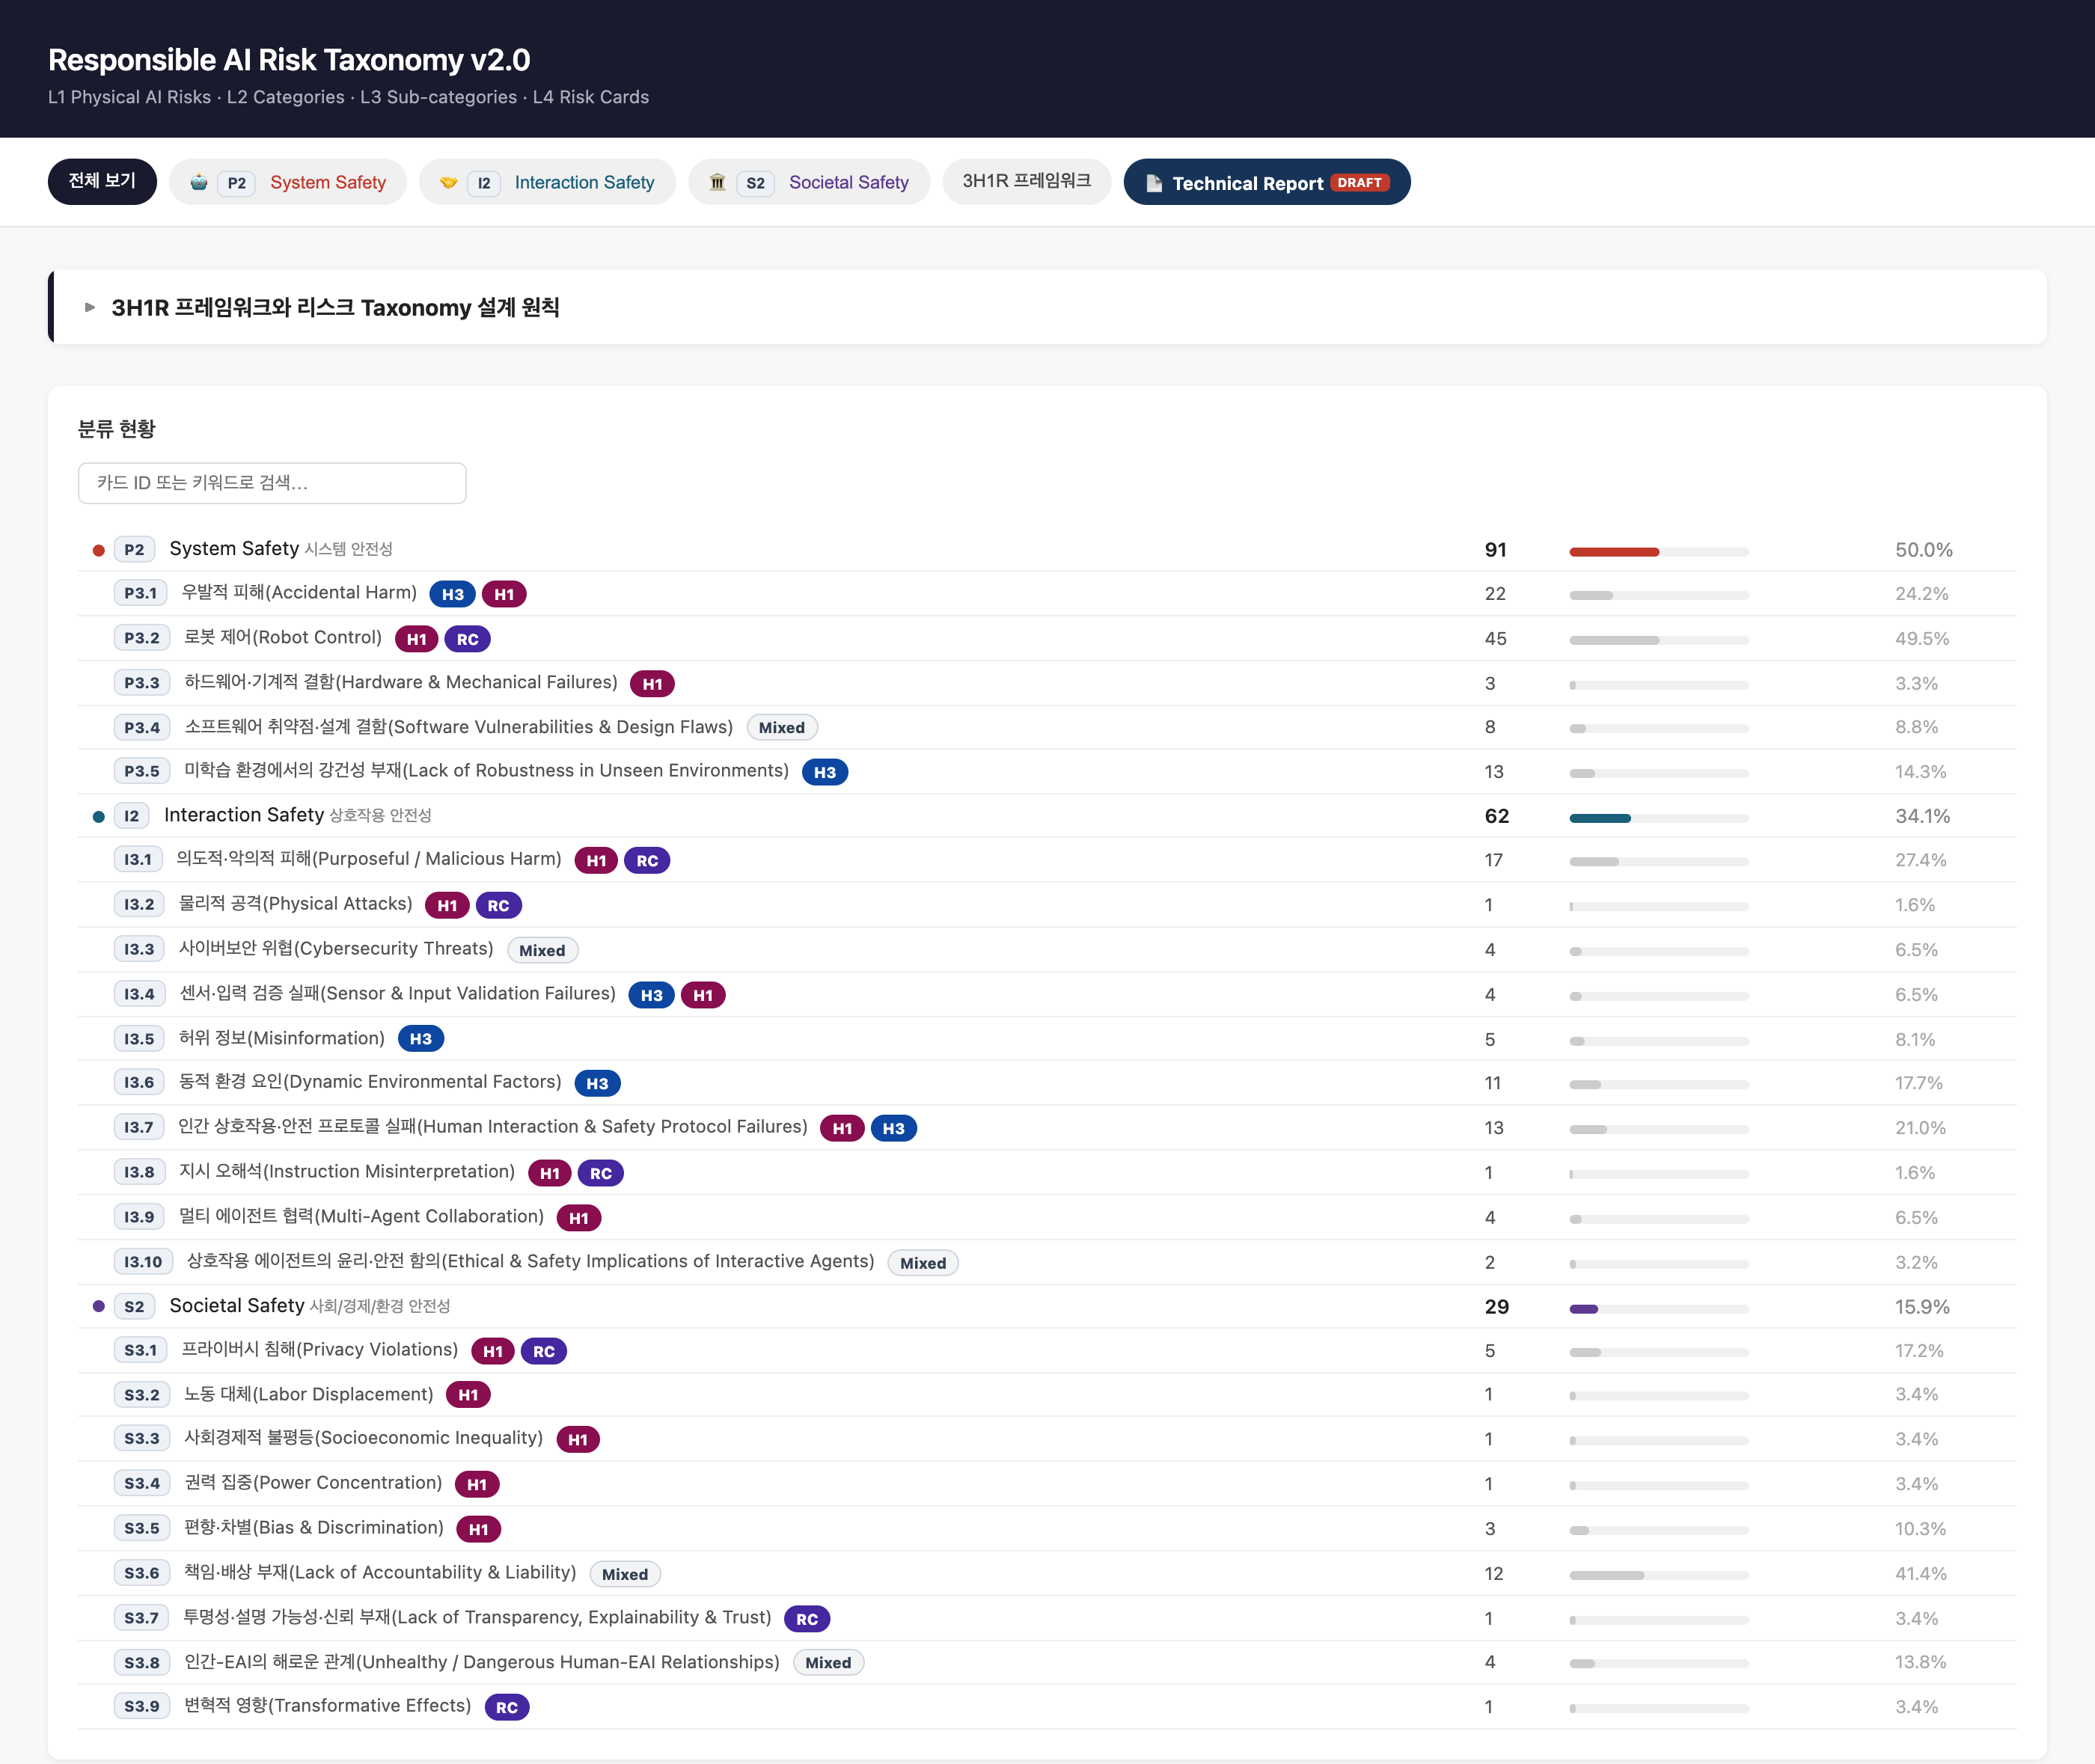
\includegraphics[width=\linewidth]{taxonomy_live_interface_1400.png}
\caption{Released taxonomy interface}
\label{fig:taxonomy-interface}
\fignote{The interface is used as the visual inspection layer for the Physical AI Risk Taxonomy. It presents the L0--L4 hierarchy, L2 source categories, L3 sub-category distribution, L4 risk-card counts, and representative 3H1R badges. The screenshot is included as a visual artifact of the release state; the report does not rely on the web page as a bibliographic source.}
\end{figure}

\section{Background: From Asimov's Laws to Alignment-Grounded Risk Cards}

The problem of constraining a physical machine's behavior did not begin with reinforcement learning; its first serious formulation is literary. Asimov's Three Laws of Robotics, together with the later Zeroth Law protecting humanity as a whole, embedded a few ranked, general-purpose priorities in the machine itself. They ask the machine to not injure a human or through inaction allow harm, to obey human orders except where they conflict with the first law, and to protect its own existence except where that conflicts with the first two~\cite{asimov1950}. The template endures, and so do its limitations. Stated in natural language, the laws are ambiguous exactly where it matters. The terms ``harm,'' ``human,'' and ``inaction'' have no operational definition a controller could evaluate, their ranking resolves conflicts only when the terms are already crisp, and they carry no representation of the machine's capability limits or of the chance that its perception is wrong. Murphy and Woods put the critique on a formal footing, arguing that the Laws are an unworkable basis for real robotics and relocating responsibility onto the humans who design and deploy the system rather than onto the robot~\cite{murphy2009}. The lesson we follow through this section is that naming priorities does not tell you how to apply them to a specific act under uncertainty.

One influential response to the brittleness of hand-specified behavior was to \emph{learn} alignment from human feedback rather than legislate it in rules. Deep reinforcement learning from human preferences established the preference-comparison mechanism that modern reinforcement learning from human feedback (RLHF) builds on, communicating goals through pairwise human judgments without a hand-coded reward~\cite{christiano2017}; instruction tuning with human feedback then scaled this to large language models (LLMs), producing assistants that follow user intent and, on the authors' evaluations, reduce toxic output~\cite{ouyang2022}. This is the practical machinery behind today's helpful--harmless--honest assistants.

Learning the objective, however, does not escape the specification problem; it inherits it. Russell frames the fixed-objective ``standard model'' of AI as the root difficulty, since a machine that optimizes a given objective perfectly will pursue it past the point its designers intended~\cite{russell2019}. Agents duly satisfy the letter of a \emph{learned} reward while violating its intent~\cite{amodei2016}, and a systematic survey documents RLHF's open problems, which range from misspecified and inconsistent human feedback to reward-model misgeneralization and the limited scalability of human oversight~\cite{casper2023}. A second limit is structural. RLHF as used to align language models operates over \emph{text}, so it does not, by itself, represent embodied action, irreversible physical consequence, or the authority a machine holds. A model can produce a perfectly polite, ``harmless''-sounding plan and still execute a motion that exceeds a joint or payload limit, grasp a blade by its edge, or compose two individually safe motions into a collision, all failures a transcript-level reward cannot see~\cite{sermanet-asimov,asimov2}.

Principle-based alignment sits \emph{on top of} feedback rather than replacing it, since a few written principles supply the targets that optimization aims at. The helpful--harmless--honest desiderata~\cite{askell2021} and constitutional training, which generates feedback from a written constitution and so reduces reliance on human preference labels~\cite{bai2022}, operationalize this for language models. Physical AI needs one axis more. We extend the three desiderata with an explicit \emph{Role Consistency} (RC) dimension, meaning behavior that stays within the authority and control boundary granted to the machine, and call the combined set \textbf{3H1R}. Role consistency is added rather than folded into Harmlessness because authority violations occur even when no physical harm results; it is the operational descendant of Asimov's obedience law.

A parallel governance line moved control from the action to the model. Capability-threshold frameworks gate deployment on whether a system crosses a dangerous-capability tier~\cite{openai2025prep,anthropic2024rsp,deepmind2025fsf}. This is the right instrument for frontier risk but coarse for Physical AI, where the failures that injure people are per-action and per-context rather than properties of a tier, since a well-below-threshold policy can still crush a hand through a mundane control error. Functional-safety engineering supplies per-failure rigor. The safety of the intended functionality (SOTIF) addresses hazards from performance limitations and foreseeable misuse absent any fault, and goal-based safety cases structure the argument for autonomous products~\cite{iso21448,ul4600}. Yet both were shaped around engineered, specifiable systems and map awkwardly onto learned policies whose failures are emergent and semantic rather than enumerable at design time~\cite{achiam2017}. The taxonomy literature is itself split. Top-down expert taxonomies give stable structure but lag the field and reflect their authors' priors~\cite{weidinger2021,hendrycks2023}, while bottom-up corpus mining captures breadth and currency but yields flat, overlapping inventories without a defensible hierarchy~\cite{slattery2024}. Neither suffices alone.

Across all of these paradigms the same seam reopens. Rules name priorities but cannot apply them under uncertainty; learned rewards inherit specification gaming and, as deployed, see only text; written principles, 3H1R included, say \emph{which} values should hold but not \emph{how} to hold a specific physical action to them, that is, how to evaluate the behavior against a value, trace it to evidence, estimate its severity, and record it as a reusable unit. Emerging embodied-safety benchmarks supply valuable test items but not that unit~\cite{sermanet-asimov,asimov2}. We supply it directly, through two commitments that organize the rest of this report. The atomic unit is the \textbf{risk card}, a single identifiable failure mode with an operational definition, supporting evidence, severity and probability estimates, and 3H1R tags, auditable in a way a natural-language law or a scalar reward is not. The construction is \textbf{hybrid}, pairing an expert-defined upper structure with corpus-derived candidates, because an expert-only taxonomy reproduces the a-priori blind spots that undid the Three Laws, while a corpus-only taxonomy inherits the ``whatever the data contains'' misgeneralization of learned objectives. Reconciling the two is the method-level form of the values-versus-evidence tension this section has tracked throughout.

\subsection*{Contributions}

\textit{Theoretical.} We recast the helpful--harmless--honest desiderata as an operational lens for embodied action and add an explicit Role Consistency axis (3H1R) that captures authority- and control-boundary failures invisible to a harm-only reading and absent in text-only settings. We give a constrained-optimization account of the Harmless--Helpful trade-off (Section~\ref{sec:hh}): modeling an embodied policy as a constrained Markov decision process~\cite{altman1999,achiam2017}, efficiency pressure predictably drives behavior toward the high-capability, high-harm quadrant, making the taxonomy's most dangerous cell a consequence of how these systems are optimized rather than an anomaly.

\textit{Methodological.} A hybrid corpus-to-taxonomy pipeline reconciles a human-defined upper structure (L0--L2 and 24 human-defined L3 families) with bottom-up candidates discovered by BGE-M3 embedding and HDBSCAN clustering over papers, policy reports, and patents; each of the 182 L4 cards is reference-grounded and auditable at the level of the individual failure mode; and an EM-style hierarchy assignment places cards under L3 with reported reproducibility and robustness checks, so the hierarchy is measured rather than asserted.

\textit{Practical.} We release an auditable 182-card catalogue with bilingual (Korean/English) coverage and 3H1R tags, usable as a governance checklist, an evaluation and red-teaming reference, and a benchmarking scaffold for Physical AI, connected to emerging embodied-safety benchmarks~\cite{sermanet-asimov,asimov2}.

\section{Prior Methodological Basis}

The source- and institution-level measures used later in this report follow four established lines of work. Bibliometric and science-mapping methods read publication metadata to describe research fields~\cite{zupic2015,vaneck2010,aria2017}, while responsible-metrics guidance cautions that organization counts should inform expert judgment rather than serve as quality rankings~\cite{hicks2015}. We therefore treat affiliation counts and PATSTAT\footnote{PATSTAT: the EPO Worldwide Patent Statistical Database, the primary patent-statistics source used in this report.} applicant counts~\cite{oecd2009patent,oecd-ipstats} as a provenance and credibility diagnostic of which universities, firms, agencies, and standards bodies appear in the corpus, and for policy and gray-literature sources we keep the issuing institutions and give more weight to high-authority bodies such as NIST, OECD, and ISO~\cite{aacods,tricco2018}, leaving quality judgments to the risk-card evidence review.

\subsection*{Prior work on constructing AI, Physical-AI, and agentic-AI risk taxonomies}

Beyond bibliometric grounding, this report builds directly on a mature line of work that turns the scholarly and policy literature into structured risk \emph{categories}. The closest methodological precedent is the MIT AI Risk Repository~\cite{slattery2024}, which applies best-fit framework synthesis to 43 existing risk frameworks, codes roughly 1{,}600 risk mentions into about 700 risks, and releases a two-level domain taxonomy (seven domains and twenty-four subdomains) alongside a causal taxonomy. This literature-to-taxonomy design, in which evidence-derived candidate risks are reconciled against an expert upper structure, is the same principle this report follows for L4 discovery and L3 assignment. Comparable literature-synthesis taxonomies include the DeepMind taxonomy of language-model risks (six areas, twenty-one risks)~\cite{weidinger2021}, the Center for AI Safety overview of catastrophic risks (four source-based categories)~\cite{hendrycks2023}, and the Stanford foundation-model risk survey~\cite{bommasani2021}.

A second group derives categories analytically or through expert policy consensus rather than corpus coding. This group includes the classic accident taxonomy of Amodei et al.~\cite{amodei2016}, the pathways matrix of Yampolskiy~\cite{yampolskiy2016}, the existential-safety delegation framework of Critch and Krueger~\cite{critch2020}, the OECD framework for classifying AI systems~\cite{oecd2022class} and its incident-terminology work~\cite{oecd2024incidents}, the NIST AI Risk Management Framework~\cite{nist-airmf}, the MITRE ATLAS adversarial-threat knowledge base~\cite{mitre-atlas}, and the extreme-risk evaluation and advanced-assistant analyses from DeepMind~\cite{shevlane2023,gabriel2024}. A third group of frontier-lab governance frameworks, such as the OpenAI Preparedness Framework~\cite{openai2025prep}, the Anthropic Responsible Scaling Policy~\cite{anthropic2024rsp}, the DeepMind Frontier Safety Framework~\cite{deepmind2025fsf}, and constitutional harm principles~\cite{bai2022}, organizes risk by capability thresholds and informs the 3H1R marking used here. For the physical and agentic setting specifically, this report draws on autonomous-system safety standards~\cite{iso21448,ul4600} and on the agentic-AI risk and governance literature~\cite{chan2023,shavit2023,chan2024,benton2024}. Table~\ref{tab:prior-taxonomies} summarizes these works together with the actual top-level categories each released, which situates the present 3-level (L1--L3) $\times$ 182-card (L4) taxonomy within established practice.

{\footnotesize
\setlength{\extrarowheight}{2pt}
\begin{longtable}{@{}p{2.15cm}p{1.7cm}p{3.5cm}p{6.35cm}@{}}
\caption{Prior risk-taxonomy work and its released top-level categories}
\label{tab:prior-taxonomies}\\
\toprule
Reference & Institution & Construction method & Released top-level categories (size) \\
\midrule
\endfirsthead
\multicolumn{4}{@{}l}{\footnotesize\itshape Table~\ref{tab:prior-taxonomies} (continued)}\\
\toprule
Reference & Institution & Construction method & Released top-level categories (size) \\
\midrule
\endhead
\midrule
\multicolumn{4}{r@{}}{\footnotesize\itshape continued on next page}\\
\endfoot
\bottomrule
\endlastfoot
\multicolumn{4}{@{}l}{\textbf{A. Literature / bibliographic synthesis taxonomies}}\\[2pt]
Slattery et al.\ 2024~\cite{slattery2024} & MIT & Meta-review of 43 frameworks ($\sim$700 coded risks) & Causal taxonomy $+$ domain taxonomy (7 domains $\times$ 24 subdomains) \\
Weidinger et al.\ 2021~\cite{weidinger2021} & DeepMind & Structured review of LM harms & Discrimination; information hazards; misinformation; malicious uses; HCI; environmental/socioeconomic (6 areas, 21 risks) \\
Hendrycks et al.\ 2023~\cite{hendrycks2023} & CAIS & Narrative synthesis by source & Malicious use; AI race; organizational; rogue AIs (4) \\
Bommasani et al.\ 2021~\cite{bommasani2021} & Stanford CRFM & Foundation-model risk survey & 7 thematic areas (fairness, misuse, environment, legality, economics, security) \\
\midrule
\multicolumn{4}{@{}l}{\textbf{B. Analytic / policy classification frameworks}}\\[2pt]
Amodei et al.\ 2016~\cite{amodei2016} & Google Brain / OpenAI & Accident classes by failure source & Side effects; reward hacking; scalable oversight; safe exploration; distributional shift (5) \\
Yampolskiy 2016~\cite{yampolskiy2016} & U.\ Louisville & Two-axis analytic matrix & Timing (pre/post-deployment) $\times$ cause \\
Critch \& Krueger 2020~\cite{critch2020} & UC Berkeley CHAI & Delegation-structure typology & Prepotent-AI types; single/multi principal $\times$ agent (29 directions) \\
OECD 2022~\cite{oecd2022class} & OECD & Policy classification of AI systems & People \& planet; economy; data; model; task/output (5 dimensions) \\
NIST 2023~\cite{nist-airmf} & NIST & Consensus framework & 7 trustworthiness traits; GOVERN/MAP/MEASURE/MANAGE \\
MITRE ATLAS~\cite{mitre-atlas} & MITRE & ATT\&CK-style attack knowledge base & Adversarial tactics matrix ($\sim$16 tactics, $\sim$84 techniques) \\
OECD 2024~\cite{oecd2024incidents} & OECD & Incident-terminology consensus & Incident vs.\ hazard; harm types (physical$\ldots$psychological) \\
Shevlane et al.\ 2023~\cite{shevlane2023} & DeepMind & Extreme-risk evaluation & Dangerous-capability $+$ alignment evaluations (2 axes) \\
Gabriel et al.\ 2024~\cite{gabriel2024} & DeepMind & Advanced-assistant monograph & Value alignment; safety; misuse; manipulation; well-being (thematic) \\
\midrule
\multicolumn{4}{@{}l}{\textbf{C. Frontier-lab capability-threshold governance frameworks}}\\[2pt]
OpenAI 2025~\cite{openai2025prep} & OpenAI & Capability thresholds (v2) & Biological/chemical; cybersecurity; AI self-improvement (3) \\
Anthropic 2023--25~\cite{anthropic2024rsp} & Anthropic & AI Safety Levels (biosafety analogue) & ASL-1--4+ tiers (CBRN uplift, autonomy) \\
DeepMind 2025~\cite{deepmind2025fsf} & DeepMind & Critical Capability Levels (v2) & CBRN; cybersecurity; ML R\&D; deceptive alignment (4) \\
Bai et al.\ 2022~\cite{bai2022} & Anthropic & Written constitution $+$ RLAIF & Helpful, harmless, honest via $\sim$16 principles \\
\midrule
\multicolumn{4}{@{}l}{\textbf{D. Physical-AI / autonomous-system risk taxonomies}}\\[2pt]
ISO 21448:2022~\cite{iso21448} & ISO & SOTIF hazard analysis & Functional insufficiencies; triggering conditions; foreseeable misuse (4 areas) \\
ANSI/UL 4600~\cite{ul4600} & UL & Goal-based safety case & Claim-based argument over $\sim$10 lifecycle topics \\
\midrule
\multicolumn{4}{@{}l}{\textbf{E. Agentic-AI risk / governance taxonomies}}\\[2pt]
Chan et al.\ 2023~\cite{chan2023} & Mila / Cambridge & Agency-feature analysis & Underspecification; directness; goal-directedness; long-term planning (4) \\
Shavit et al.\ 2023~\cite{shavit2023} & OpenAI & Lifecycle governance practices & 7 practices (task-suitability $\ldots$ interruptibility) \\
Chan et al.\ 2024~\cite{chan2024} & GovAI / Mila & Agent-visibility measures & Agent identifiers; real-time monitoring; activity logging (3) \\
Benton et al.\ 2024~\cite{benton2024} & Anthropic & Sabotage threat model $+$ evals & Human-decision; code; sandbagging; undermining oversight (4) \\
\end{longtable}
\vspace{-4pt}
{\footnotesize\itshape Abbreviations:} {\footnotesize CBRN, chemical/biological/radiological/nuclear; ASL, AI Safety Levels; RLAIF, reinforcement learning from AI feedback; SOTIF, safety of the intended functionality; ML R\&D, machine-learning research and development.}
}


\section{Design Requirements and Release Controls}

This Technical Report operationalizes a hybrid Physical AI risk-taxonomy design: the upper levels (L0--L3) are stabilized through top-down governance logic, while L4 risk cards are generated from a bottom-up evidence corpus and then mapped back to the hierarchy. Table~\ref{tab:design-requirements} records how each design requirement is implemented and where it is substantiated in this report.

\begin{table}[htbp]
\centering
\footnotesize
\caption{Design requirements and their substantiation}
\label{tab:design-requirements}
\begin{tabularx}{\linewidth}{p{0.30\linewidth}X}
\toprule
Design requirement & Where it is substantiated \\
\midrule
Taxonomy design: near-MECE, standard-aligned terms, hybrid top-down/bottom-up construction. & Scope, prior-basis, and workflow sections define the L0--L4 hierarchy, 3H1R rules, and an auditable workflow separating collection, clustering, reference grounding, review, and release. \\
Hierarchy: fix L0--L3 before L4 mapping (L1 Physical AI, three L2 categories, 24 L3). & Scope and released-hierarchy sections document L0--L4 structure, L2/L3 coverage, and the rule that every L3 keeps \(\geq 1\) L4 after review. \\
Source collection: build the AI corpus from Web of Science (WoS), policy reports, and PATSTAT; select Physical AI via BGE-M3 anchors plus explicit terms; keep risk records by safety/failure terms. & Data-sources section reports the integrated corpus (Table~\ref{tab:integrated-document-space-counts}); Appendices A--C give the PATSTAT SQL, Physical AI/risk filters, and the Web of Science query. \\
L4 discovery: HDBSCAN clustering, c-TF-IDF keyphrases, reference-grounded candidates, iterative merge at cosine \(\geq 0.94\). & Risk-candidate section and Algorithm~1 formalize embedding, clustering, labeling, the reference filter, and the merge rule, yielding the 182-card L4 set. \\
Card schema: layer-based stable IDs; bilingual fields, hierarchy, references, severity/probability; new cards need independent references, semantic distance, and a valid L2. & Generation and card-schema sections specify ID prefixes, required fields, the five-reference cap, duplicate exclusion, and release validation. \\
L3 mapping: with seeds, assign each L4 to the nearest L3 and check alternatives; without seeds, induce L3 families from clusters of three or more L4 risks. & L3-assignment section and Algorithm~2 formalize seeded assignment, EM-style centroid update, and the bottom-up induction fallback. \\
3H1R application: read Helpful, Harmless, Honest, and Role Consistency as behavior, safety-constraint, world-state, uncertainty, and role-boundary failures. & 3H1R section operationalizes 3H1R, defines Primary/Secondary causal-proximity rules, and separates L4 coding from L3 icons. \\
\bottomrule
\end{tabularx}
\end{table}

Two threshold choices are treated as explicit release controls. First, the 0.52 Physical AI similarity threshold is paired with lexical overrides and audit inspection of below-threshold domains dominated by out-of-scope records such as nursing, agriculture, tourism, and general medical documents. Second, the 0.94 merge threshold is treated as an empirical separation point in the candidate-similarity distribution. It is intentionally conservative: a lower threshold would collapse distinct Physical AI failure modes, while a higher threshold would leave near-duplicate risk cards unresolved.

\section{Workflow Overview}

Figure~\ref{fig:workflow} summarizes the end-to-end workflow from raw source collection to the released taxonomy artifacts. The pipeline is hybrid: corpus-derived evidence generates and deduplicates L4 risk candidates, while authoritative references and human review stabilize the hierarchy, definitions, and evidence justifications.

For reproducibility, each stage is documented as an auditable transformation rather than as a narrative judgment. The raw retrieval layer is preserved through the exact PATSTAT SQL and Web of Science topic query reproduced in Appendices~A and~B. The intermediate layer records source-family counts, local file names, row counts, column counts, and file sizes. The modeling layer specifies the embedding input text, clustering method, c-TF-IDF label extraction, reference-grounding rule, merge threshold, and L3 assignment rule. The release layer is exported from the final HTML into CSV/JSON files so that card counts, references, hierarchy assignments, and 3H1R tags can be checked independently from the rendered web page.

\begin{figure}[htbp]
\centering
\resizebox{\linewidth}{!}{%
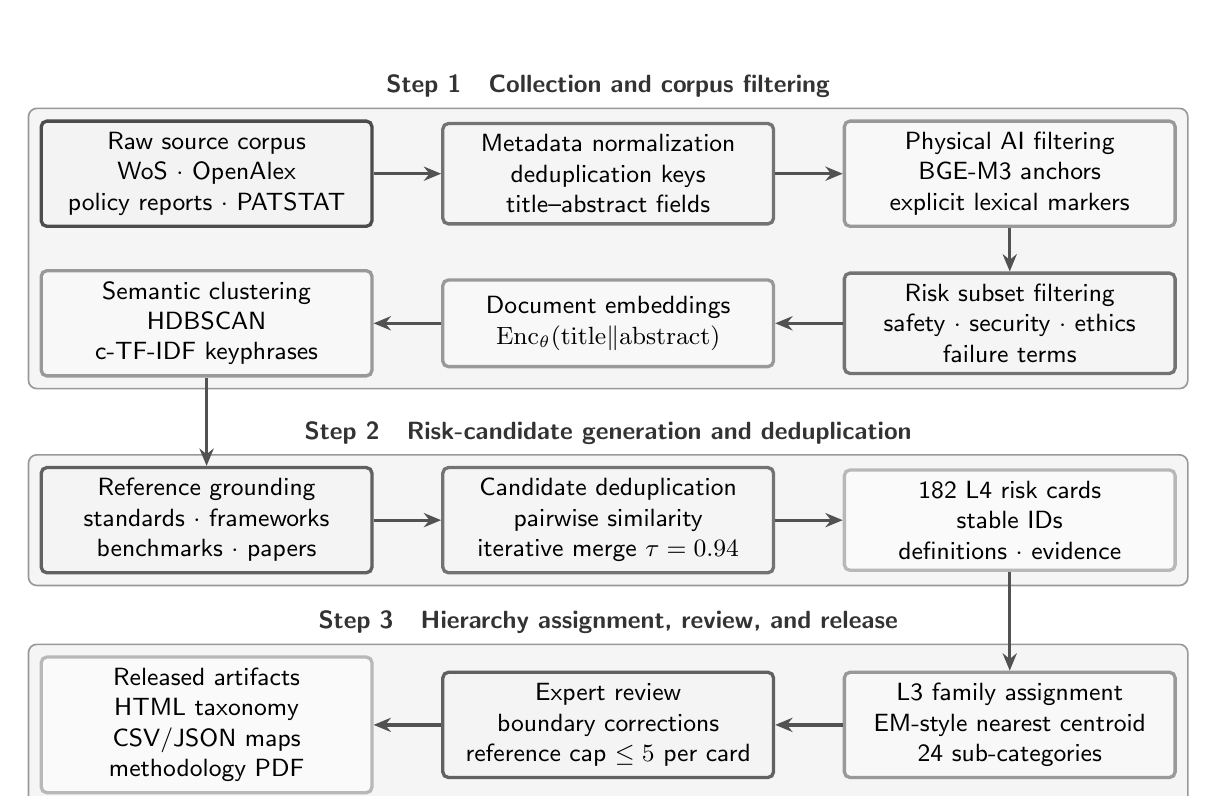
\begin{tikzpicture}[
  font=\sffamily\small,
  node distance=8mm and 10mm,
  box/.style={rectangle, rounded corners=2pt, draw=#1, very thick, fill=#1!7,
    align=center, minimum width=42mm, minimum height=11mm, inner sep=4pt},
  proc/.style={box=flowg1},
  data/.style={box=flowg2},
  model/.style={box=flowg3},
  review/.style={box=flowg4},
  outputbox/.style={box=flowg5},
  arrow/.style={-{Stealth[length=2.2mm,width=1.8mm]}, very thick, draw=black!68}
]

\node[data] (sources) at (0,0) {Raw source corpus\\WoS \(\cdot\) OpenAlex\\policy reports \(\cdot\) PATSTAT};
\node[proc] (normalize) at (5.1,0) {Metadata normalization\\deduplication keys\\title--abstract fields};
\node[model] (anchors) at (10.2,0) {Physical AI filtering\\BGE-M3 anchors\\explicit lexical markers};

\node[proc] (riskfilter) at (10.2,-1.9) {Risk subset filtering\\safety \(\cdot\) security \(\cdot\) ethics\\failure terms};
\node[model] (embed) at (5.1,-1.9) {Document embeddings\\\(\Enc(\mathrm{title}\Vert\mathrm{abstract})\)};
\node[model] (cluster) at (0,-1.9) {Semantic clustering\\HDBSCAN\\c-TF-IDF keyphrases};

\node[review] (reffilter) at (0,-4.4) {Reference grounding\\standards \(\cdot\) frameworks\\benchmarks \(\cdot\) papers};
\node[proc] (merge) at (5.1,-4.4) {Candidate deduplication\\pairwise similarity\\iterative merge \(\tau=0.94\)};
\node[outputbox] (l4) at (10.2,-4.4) {182 L4 risk cards\\stable IDs\\definitions \(\cdot\) evidence};

\node[model] (l3) at (10.2,-7.0) {L3 family assignment\\EM-style nearest centroid\\24 sub-categories};
\node[review] (human) at (5.1,-7.0) {Expert review\\boundary corrections\\reference cap \(\leq 5\) per card};
\node[outputbox] (release) at (0,-7.0) {Released artifacts\\HTML taxonomy\\CSV/JSON maps\\methodology PDF};

\draw[arrow] (sources) -- (normalize);
\draw[arrow] (normalize) -- (anchors);
\draw[arrow] (anchors) -- (riskfilter);
\draw[arrow] (riskfilter) -- (embed);
\draw[arrow] (embed) -- (cluster);
\draw[arrow] (cluster) -- (reffilter);
\draw[arrow] (reffilter) -- (merge);
\draw[arrow] (merge) -- (l4);
\draw[arrow] (l4) -- (l3);
\draw[arrow] (l3) -- (human);
\draw[arrow] (human) -- (release);

\begin{scope}[on background layer]
  \node[draw=black!40, semithick, rounded corners=3pt, fill=black!4, inner sep=4pt,
    fit=(sources)(normalize)(anchors)(riskfilter)(embed)(cluster)] (bandA) {};
  \node[draw=black!40, semithick, rounded corners=3pt, fill=black!4, inner sep=4pt,
    fit=(reffilter)(merge)(l4)] (bandB) {};
  \node[draw=black!40, semithick, rounded corners=3pt, fill=black!4, inner sep=4pt,
    fit=(l3)(human)(release)] (bandC) {};
\end{scope}
\node[anchor=south, font=\sffamily\small\bfseries, text=black!80] at (bandA.north)
  {Step 1\quad Collection and corpus filtering};
\node[anchor=south, font=\sffamily\small\bfseries, text=black!80] at (bandB.north)
  {Step 2\quad Risk-candidate generation and deduplication};
\node[anchor=south, font=\sffamily\small\bfseries, text=black!80] at (bandC.north)
  {Step 3\quad Hierarchy assignment, review, and release};

\end{tikzpicture}%
}
\caption{End-to-end taxonomy construction and release workflow}
\label{fig:workflow}
\fignote{Arrows denote the main data-processing path. The expert-review stage is applied iteratively: L4 risk cards and L3 assignments are repeatedly revised through expert review before release.}
\end{figure}

\section{Data Sources and Corpus Construction}

The construction corpus integrates three source families: scholarly publications, policy/report documents, and patent records. Scholarly records were collected from Web of Science and related local scholarly metadata snapshots, patent records from EPO PATSTAT, and policy/report records from domestic and international policy collections~\cite{clarivate-wos,openalex,epo-patstat}. The reproducible retrieval evidence is retained in three forms, reproduced verbatim in Appendices~A--C: the Web of Science topic-search expression, the PATSTAT AI patent-retrieval SQL, and the SQL-equivalent Physical AI / Physical AI risk filtering rules. Table~\ref{tab:integrated-document-space-counts} reports the integrated corpus sizes; these are the corpus-level counts used to motivate the L4 generation pipeline.

\begin{table}[htbp]
\centering
\caption{Integrated corpus counts by source family and category}
\label{tab:integrated-document-space-counts}
\begin{tabular}{lrrrr}
\toprule
Dataset group & Papers & Policy reports & Patents & Total \\
\midrule
AI & 1,749,159 & 125,372 & 2,032,236 & 3,906,767 \\
AI Infrastructure & 219,002 & 341 & 522,085 & 741,428 \\
Physical AI & 31,386 & 1,654 & 350,109 & 383,149 \\
Physical AI Risks & 50,375 & 938 & 31,658 & 82,971 \\
\bottomrule
\end{tabular}

\par\smallskip\begin{minipage}{0.92\linewidth}
\footnotesize\textit{Note:} Counts are reported after within-group deduplication; category overlap is intentionally retained across AI, AI infrastructure, Physical AI, and Physical AI risks. The integrated datasets are organized as three source-family collections, namely papers, policy reports, and patents, each split into AI, AI infrastructure, Physical AI, and Physical AI risks. Counts exclude records without usable title text during standardization.
\end{minipage}
\end{table}

Table~\ref{tab:integrated-document-space-counts} reports the integrated corpus sizes by category and source family. Paper counts are parsed from the local Web of Science AI export, patents from the PATSTAT datasets, and policy records from the curated policy corpora, with within-group (per document type and category) deduplication and intentional cross-category overlap. Every group preserves a domestic/global key, namely applicant country for patents, Korea affiliation for papers, and a domestic/foreign flag for policy, so each figure can be reported as domestic, overseas, and total. Within the Physical AI risk group of 82,971 records, scholarly publications dominate (Web of Science, 50,375; 60.7\%), followed by patents (31,658; 38.2\%) and policy or report sources (938; 1.1\%).

To characterize provenance beyond raw counts, country and institution were back-filled for the Physical AI risk \emph{papers and policy reports} by re-joining each record to its original source (Web of Science / OpenAlex affiliations by DOI and source identifier, with OpenAlex and Crossref resolving the remaining gaps). This recovered an institution for 38,008 records (papers 73.6\%, policy 98.7\%) and a country for 36,643 records. Patents were separately enriched with applicant/assignee and country from PATSTAT (\texttt{tls207\_pers\_appln}\,$\bowtie$\,\texttt{tls206\_person} on \texttt{appln\_id}; applicant 99.6\%, country 38\%), but are deliberately excluded from the country and institution rankings below: patent-applicant counts index commercial IP-filing activity and would read as a technology-competitiveness ranking rather than research and governance attention to Physical AI risks. Tables~\ref{tab:country-top}--\ref{tab:institution-top} therefore reflect scholarly papers and policy reports; counts are document--organization and document--country links over records with a resolved affiliation, not a complete census.

\begin{table}[htbp]
\centering
\footnotesize
\caption{Country distribution of Physical AI risk records}
\label{tab:country-top}
\begin{tabular}{rlrr}
\toprule
Rank & Country & Records & Share (\%) \\
\midrule
1 & China & 7,161 & 19.5 \\
2 & United States & 6,937 & 18.9 \\
3 & India & 2,493 & 6.8 \\
\bfseries 4 & \bfseries South Korea & \bfseries 2,208 & \bfseries 6.0 \\
5 & United Kingdom & 1,697 & 4.6 \\
6 & Germany & 1,434 & 3.9 \\
7 & Italy & 1,121 & 3.1 \\
8 & Canada & 1,012 & 2.8 \\
9 & Japan & 839 & 2.3 \\
10 & Australia & 735 & 2.0 \\
11 & Spain & 648 & 1.8 \\
12 & France & 537 & 1.5 \\
13 & Saudi Arabia & 410 & 1.1 \\
14 & Netherlands & 385 & 1.1 \\
15 & Pakistan & 372 & 1.0 \\
\bottomrule
\end{tabular}

\par\smallskip\begin{minipage}{0.92\linewidth}
\footnotesize\textit{Note:} Counts are over Physical AI risk papers and policy reports with a resolved country. Patents were enriched from PATSTAT (country present for 38\% of patents) but are excluded here, because patent-applicant counts reflect commercial IP filing rather than research or governance attention and could be misread as technology competitiveness.
\end{minipage}
\end{table}

Physical AI risk activity is globally distributed and led by China, the United States, and India; Korea-affiliated records account for 6.0\% (2,208 of 36,643 records with a resolved country).

\begin{table}[htbp]
\centering
\footnotesize
\caption{Top institutions in Physical AI risk records}
\label{tab:institution-top}
\begin{tabular}{rlr}
\toprule
Rank & Institution / organization & Records \\
\midrule
1 & Tsinghua University & 177 \\
2 & Korea Advanced Institute of Science and Technology & 165 \\
3 & Shanghai Jiao Tong University & 160 \\
4 & Harbin Institute of Technology & 160 \\
5 & Technical University of Munich & 142 \\
6 & Carnegie Mellon University & 142 \\
7 & Beijing Institute of Technology & 141 \\
8 & Beihang University & 133 \\
9 & Nanyang Technological University & 132 \\
10 & Seoul National University & 132 \\
11 & University of California & 125 \\
12 & Northeastern University & 125 \\
13 & Chinese Academy of Sciences & 120 \\
14 & Tongji University & 119 \\
15 & Northwestern Polytechnical University & 117 \\
\bottomrule
\end{tabular}

\par\smallskip\begin{minipage}{0.92\linewidth}
\footnotesize\textit{Note:} Most frequent institutions/organizations over Physical AI risk papers and policy reports with a resolved affiliation. Patent applicants/assignees are excluded (enriched from PATSTAT as a backup) to avoid conflating commercial IP filing with research and governance attention.
\end{minipage}
\end{table}

The filtering logic has two stages. First, candidate Physical AI records are identified by cosine similarity to Physical AI definition anchors derived from NVIDIA, NIST, ISO, MITRE ATLAS, and ASIMOV-style embodied safety references\footnote{ASIMOV Benchmark v2: \url{https://asimov-benchmark.github.io/v2/}.} using the BGE-M3 encoder\footnote{BGE-M3 model card: \url{https://huggingface.co/BAAI/bge-m3}. The underlying M3-Embedding paper is cited in the References~\cite{chen2024bgem3}.}. These anchors cover AI risk management, industrial robot safety, functional safety, controllability, adversarial AI, world-model-based Physical AI development, and embodied semantic safety~\cite{nist-airmf,iso23894,iso10218,iso5469,iso8200,mitre-atlas,nvidia-cosmos,sermanet-asimov,asimov2}. Records with similarity above 0.52, or with explicit Physical AI terms such as \textit{physical AI}, \textit{humanoid}, \textit{embodied AI}, or cyber-physical systems (\textit{CPS}), are retained as Physical AI candidates. Second, the candidate set is filtered to records whose title or abstract contains risk, safety, failure, security, ethics, or related terms. This produces the Physical AI risk group \(|\DPAI|=82,971\). To reproduce this step, a researcher concatenates each record's title and abstract, computes the BGE-M3 embedding, compares it with the documented Physical AI anchor descriptions, applies the 0.52 threshold and lexical-marker override, and then applies the risk-term filter to the retained candidate set.

Formally, let \(\mathcal{D}_{AI}=\{d_i\}_{i=1}^{N}\) be the retrieved AI corpus and let \(x_i=\mathrm{title}(d_i)\Vert\mathrm{abstract}(d_i)\Vert\mathrm{keywords}(d_i)\) be the normalized document text. Let \(\mathcal{P}=\{p_q\}_{q=1}^{Q}\) denote Physical AI anchor descriptions derived from the authoritative sources above, and let \(\mathcal{K}_{PAI}\) and \(\mathcal{K}_{risk}\) denote the explicit Physical AI lexical markers and risk/safety lexical markers, respectively. The document and anchor embeddings are
\begin{equation}
  e_i=\frac{\Enc(x_i)}{\|\Enc(x_i)\|_2}, \qquad
  u_q=\frac{\Enc(p_q)}{\|\Enc(p_q)\|_2}.
\end{equation}
The Physical AI relevance score is the maximum anchor similarity:
\begin{equation}
  s_i^{PAI}=\max_{q\in\{1,\ldots,Q\}} e_i^{\top}u_q.
\end{equation}
A document is retained as a Physical AI candidate if
\begin{equation}
  d_i\in\mathcal{D}_{PAI}^{cand}
  \Longleftrightarrow
  \left(s_i^{PAI}\geq\tau_{PAI}=0.52\right)
  \lor
  \left[\exists k\in\mathcal{K}_{PAI}: k\subset x_i\right].
\end{equation}
The final Physical AI risk corpus is then
\begin{equation}
  \DPAI=
  \left\{d_i\in\mathcal{D}_{PAI}^{cand}:
  \exists r\in\mathcal{K}_{risk}\ \text{such that}\ r\subset x_i
  \right\}.
\end{equation}
This two-stage rule separates semantic inclusion in the Physical AI domain from risk-specific filtering. The lexical override prevents highly specific terms such as \textit{humanoid}, \textit{embodied AI}, or \textit{CPS} from being lost when a short abstract produces a lower anchor similarity score.

\section{Corpus and Taxonomy Statistics}

\textbf{Record-level snapshot.} The year-level statistics in this section are computed on a released local reproducible snapshot of 23,191 Physical AI records (7,132 scholarly, 1,042 policy, and 15,017 patent), which is the auditable slice available for direct recomputation. The full corpus totals are reported separately in Table~\ref{tab:integrated-document-space-counts} as the integrated-source view.

\textbf{Level distribution.} Figure~\ref{fig:level-dist} summarizes how the 182 released L4 risk cards distribute across the taxonomy levels. System Safety (P2) holds 92 cards (50.5\%), Interaction Safety (I2) 60 (33.0\%), and Societal Safety (S2) 30 (16.5\%). At L3, the largest families are Robot Control (46), Accidental Harm (22), and Purposeful/Malicious Harm (17), followed by Lack of Robustness in Unseen Environments (13), Lack of Accountability \& Liability (13), and Human Interaction \& Safety Protocol Failures (12). Societal families are intentionally retained even when sparse because the taxonomy supports governance review and future expansion, not only frequency-based clustering.

\begin{figure}[htbp]
\centering
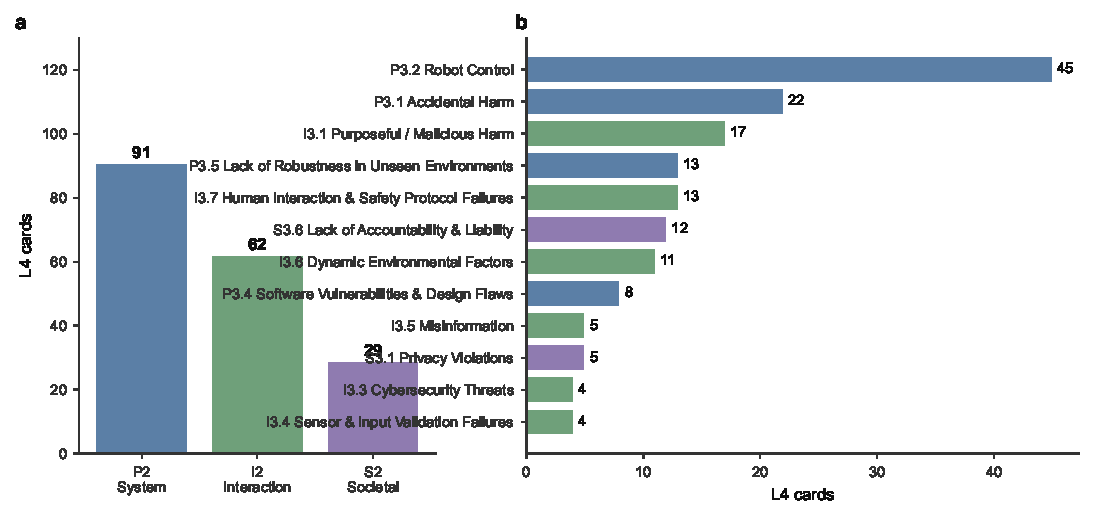
\includegraphics[width=\linewidth]{fig_taxonomy_levels.pdf}
\caption{Distribution of the 182 released L4 risk cards}
\label{fig:level-dist}
\fignote{Main panel: top L3 sub-categories by L4 card count, colored by L2 domain (blue = System, green = Interaction, purple = Societal). Inset: L2 category distribution (P2 System, I2 Interaction, S2 Societal).}
\end{figure}

\section{Document-Space Embedding and Projection}

The integrated AI document space in Figure~\ref{fig:ai-doc-space} visualizes how AI, AI infrastructure, Physical AI, and Physical AI risk evidence relate at the document level. Each document \(d\) is represented by the concatenation of its title and abstract, \(x_d=\mathrm{title}(d)\Vert\mathrm{abstract}(d)\), encoded with the BGE-M3 sentence embedder~\cite{chen2024bgem3} and \(L_2\)-normalized,
\begin{equation}
  z_d=\frac{\Enc(x_d)}{\|\Enc(x_d)\|_2},\qquad \|z_d\|_2=1,
\end{equation}
so that inner products \(z_d^{\top}z_{d'}\) equal cosine similarities. Because embedding every one of the 5.1 million records in a single vector space is limited by available compute, the figure embeds a 1\% stratified random sample drawn at the same rate from each source-family and category stratum of the full corpus under a fixed seed. Applying one common rate to every stratum keeps the plotted point counts proportional to the Table~\ref{tab:integrated-document-space-counts} populations, and the sample spans all years rather than a recent window.

\begin{figure}[htbp]
\centering
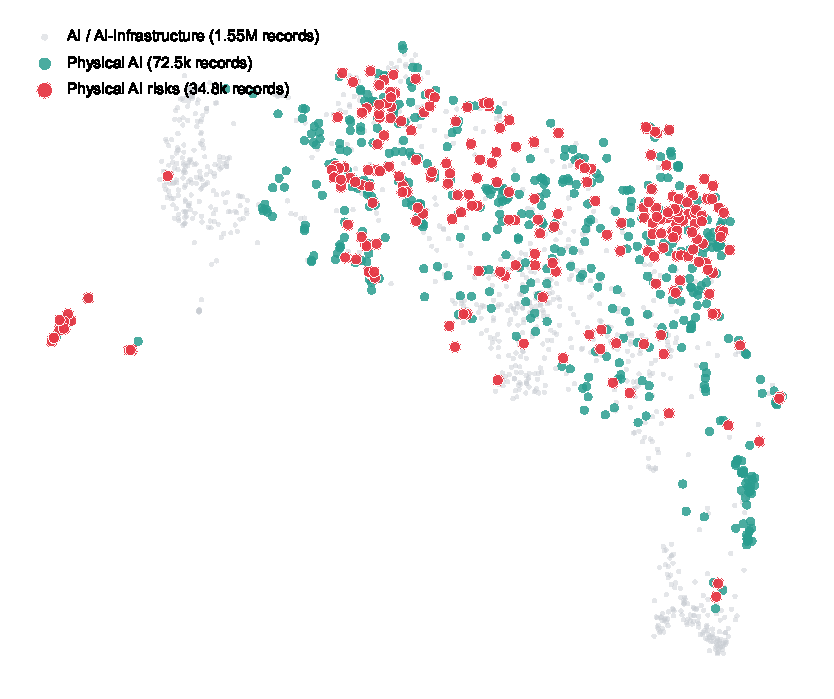
\includegraphics[width=0.9\linewidth]{fig_recent_physical_ai_space.pdf}
\caption{Physical AI document space (1\% stratified sample of the full corpus, all years)}
\label{fig:ai-doc-space}
\fignote{The figure embeds a 1\% stratified random sample of the full integrated corpus, about 50{,}991 of 5{,}099{,}045 records, drawn at the same rate from every source-family and category stratum so the plotted counts stay proportional to Table~\ref{tab:integrated-document-space-counts} across all years. Text is embedded with BGE-M3 (title\,+\,abstract) and projected with UMAP (fixed seed 20260704). The AI records are further split by title keywords into a vision group (6{,}233 points) and a broadly defined language group (1{,}408 points, covering natural-language processing, large language and foundation models, and generative text work), with the remaining general AI work (31{,}318 points) and AI infrastructure (7{,}395 points) forming a neutral backdrop. AI infrastructure is drawn in pure grey and the general AI work in a very light grey, while the vision and language groups carry blue and green tints so the two can be compared. Physical AI (3{,}807 points) and Physical AI risks (830 points) share one warm family, with Physical AI in coral and the risk layer drawn on top in a deep crimson. Read against the two coloured groups, the risk points fall predominantly in and around the vision region rather than the language region.}
\end{figure}

The sampled embeddings are projected to two dimensions with uniform manifold approximation and projection (UMAP)~\cite{umap2018}. UMAP first builds a weighted \(k\)-nearest-neighbor graph: for point \(i\) with neighbor \(j\), the directed membership is
\begin{equation}
  p_{j\mid i}=\exp\!\left(-\frac{\max(0,\,d(z_i,z_j)-\rho_i)}{\sigma_i}\right),
\end{equation}
where \(d\) is the cosine distance, \(\rho_i\) is the distance to \(i\)'s nearest neighbor, and \(\sigma_i\) is set so that \(\sum_j p_{j\mid i}=\log_2 k\). Directed memberships are symmetrized as \(p_{ij}=p_{j\mid i}+p_{i\mid j}-p_{j\mid i}\,p_{i\mid j}\). A low-dimensional layout \(\{y_i\}\subset\mathbb{R}^2\), with membership \(q_{ij}=(1+a\|y_i-y_j\|_2^{2b})^{-1}\), is optimized by minimizing the fuzzy-set cross-entropy
\begin{equation}
  \mathcal{C}=\sum_{i\neq j}\left[p_{ij}\log\frac{p_{ij}}{q_{ij}}+(1-p_{ij})\log\frac{1-p_{ij}}{1-q_{ij}}\right],
\end{equation}
which preserves local neighborhood structure while allowing globally distinct groups to separate. Points are colored by dataset group and marked by document type; the sample index, embeddings, and 2D coordinates are stored with the integrated dataset so that the figure is fully reproducible.

\section{Risk Candidate Generation and Deduplication}

The L4 generation stage transforms heterogeneous documents into semantically coherent risk candidates. Documents are embedded using BGE-M3 from title and abstract fields~\cite{chen2024bgem3}. Hierarchical density-based spatial clustering of applications with noise (HDBSCAN) is applied to the embedding space to identify clusters of semantically coherent risk evidence~\cite{campello2013,hdbscan2017}. Let \(E=\{e_i\}_{i=1}^{|\DPAI|}\) be the unit-normalized document embeddings for the retained Physical AI risk corpus. The base semantic distance is cosine distance:
\begin{equation}
  \delta(i,j)=1-e_i^{\top}e_j.
\end{equation}
For HDBSCAN, let \(c_k(i)\) denote the core distance from point \(i\) to its \(k\)-th nearest neighbor. The mutual reachability distance used to build the density hierarchy is
\begin{equation}
  d_{\mathrm{mreach},k}(i,j)=
  \max\{c_k(i),c_k(j),\delta(i,j)\}.
\end{equation}
HDBSCAN constructs a minimum spanning tree over \(d_{\mathrm{mreach},k}\), condenses the resulting hierarchy by minimum cluster size, and selects clusters with high persistence. The output is a partial assignment
\begin{equation}
  h:\mathcal{D}_{PAI}\rightarrow\{1,\ldots,M\}\cup\{-1\},
\end{equation}
where \(h(d_i)=m\) means that document \(d_i\) belongs to risk-evidence cluster \(C_m\), and \(h(d_i)=-1\) denotes density noise. Noise points are not discarded automatically; they can later be recovered by direct reference matching or expert review.

For each cluster \(C_m\), class-based term frequency--inverse document frequency (c-TF-IDF) extracts representative keyphrases, following the topic-representation logic of BERTopic~\cite{grootendorst2022}:
\begin{equation}
  \mathrm{cTFIDF}(t,C_m)=
  \frac{f_{t,C_m}}{|C_m|}
  \cdot
  \log
  \frac{|\DPAI|}{\sum_{m'} f_{t,C_{m'}}}.
\end{equation}
The top-\(k\) keyphrases become raw risk labels. Candidate labels are retained only when they can be grounded in an authoritative reference corpus or a direct citation link. The authoritative corpus includes AI risk-management standards, robotics safety standards, adversarial-AI knowledge bases, and embodied-AI benchmarks~\cite{nist-airmf,iso23894,iso10218,iso5469,iso8200,mitre-atlas,sermanet-asimov,asimov2}. This reference filter reduces noisy cluster labels and ensures that each candidate is auditable. If \(a_b\in\mathcal{A}\) is an authoritative reference text and \(\ell_m\) is the raw cluster label, the semantic grounding score is
\begin{equation}
  g_m=\max_{a_b\in\mathcal{A}}
  \simcos\!\left(\Enc(\ell_m),\Enc(a_b)\right).
\end{equation}
The retained candidate set is
\begin{equation}
  C_0=\{c_m:g_m\geq\tau_{\mathrm{ref}}\ \lor\ \mathrm{directCitation}(c_m)=1\}.
\end{equation}

The reference-filtered candidates are then embedded again using label and definition text. For each \(c_j\in C_0\), define \(v_j=\Enc(\mathrm{label}(c_j)\Vert\mathrm{definition}(c_j))\) and normalize \(v_j\) to unit length. Pairwise cosine similarity is
\begin{equation}
  S_{jk}=v_j^{\top}v_k,\qquad j\neq k.
\end{equation}
Deduplication is a constrained agglomerative merge over candidate nodes. At iteration \(t\), choose
\begin{equation}
  (j^{\ast},k^{\ast})=\arg\max_{j\neq k}S_{jk}.
\end{equation}
If \(S_{j^{\ast}k^{\ast}}\geq\tau_{\mathrm{merge}}=0.94\), the two candidates are replaced by a canonical node
\begin{equation}
  c_{j^{\ast}}\leftarrow
  \mathrm{merge}(c_{j^{\ast}},c_{k^{\ast}})
  =
  \bigl(\mathrm{richerDefinition},\
  \mathrm{evidence}_{j^{\ast}}\cup\mathrm{evidence}_{k^{\ast}},\
  \mathrm{refs}_{j^{\ast}}\cup\mathrm{refs}_{k^{\ast}}\bigr),
\end{equation}
and \(c_{k^{\ast}}\) is removed. The affected similarity row and column are recomputed from the updated label-definition text. The algorithm stops when \(\max_{j\neq k}S_{jk}<0.94\). The threshold is treated as an empirical distribution cut point: lower values collapse distinct risk types, while higher values leave near-duplicate cards.

\begin{algobox}{Algorithm 1. Risk Candidate Generation and Deduplication Pipeline}
\begin{enumerate}[leftmargin=1.6em,itemsep=0.35em]
  \item \textbf{Input:} Tri-domain Physical AI risk corpus \(\DPAI\), with \(|\DPAI|=82,971\) records (50,375 scholarly records, 938 policy/report records, and 31,658 patents); BGE-M3 encoder \(\Enc\)~\cite{chen2024bgem3}; and an authoritative reference corpus \(\mathcal{A}\) containing standards, risk frameworks, benchmarks, and high-quality papers~\cite{nist-airmf,iso23894,iso10218,mitre-atlas,sermanet-asimov}.
  \item \textbf{Normalize records:} Retain source identifier, title, abstract, year, DOI or URL, source family, and retrieval provenance. Remove exact duplicate records using DOI where available, otherwise title--URL keys.
  \item \textbf{Embed documents:} For each \(d_i \in \DPAI\), compute \(e_{d_i} \leftarrow \Enc(\mathrm{title}(d_i) \Vert \mathrm{abstract}(d_i))\). Empty abstracts are represented by title-only text and flagged in the metadata.
  \item \textbf{Cluster:} Apply HDBSCAN to \(\{e_{d_i}\}\) and obtain semantically coherent clusters \(\{C_1,\ldots,C_M\}\)~\cite{campello2013,hdbscan2017}. Treat noise points as unassigned evidence unless later recovered by direct reference matching.
  \item \textbf{Extract keyphrases:} For each \(C_m\), compute c-TF-IDF and extract the top-\(k\) terms as the raw risk label \(\ell_m\)~\cite{grootendorst2022}.
  \item \textbf{Reference filter:} Retain \(\ell_m\) if an authoritative source \(a \in \mathcal{A}\) satisfies \(\simcos(e_{\ell_m},e_a)\geq\tau_{\mathrm{ref}}\), or if a direct citation link exists. The retained raw candidate set is \(C_0\), with \(|C_0|=812\). Store the matched reference, similarity score or citation link, and a short evidence sentence.
  \item \textbf{Embed candidates:} For each candidate \(c_j \in C_0\), compute \(e_{c_j}\leftarrow\Enc(\mathrm{label}(c_j)\Vert\mathrm{definition}(c_j))\).
  \item \textbf{Pairwise similarity:} Compute \(S_{jk}=\simcos(e_{c_j},e_{c_k})\) for all \(j\neq k\).
  \item \textbf{Iterative merging:} While there exists a pair \((j,k)\) such that \(S_{jk}\geq\tau_{\mathrm{merge}}=0.94\), select the highest-similarity pair, merge it into a canonical node by unioning evidence and retaining the richer definition, remove the redundant node, and update the affected row and column of \(S\).
  \item \textbf{Human audit:} Review high-similarity non-merged pairs, low-reference candidates, and candidates whose evidence does not support the proposed risk definition. Remove unsupported candidates or rewrite definitions before release.
  \item \textbf{Output and checks:} Export 182 unique L4 risk cards. Verify stable IDs, no duplicate DOI/title/URL references within a card, at most five references per card, and a non-empty bilingual definition and evidence justification for each released card.
\end{enumerate}
\end{algobox}

\section{Card Schema and Identifier Assignment}

Each retained L4 risk is converted into a card with a stable identifier and a structured schema. The identifier prefix records the primary evidence layer: \texttt{PHYSRISK} for standards/frameworks, \texttt{PHYSBENCH} for benchmarks, \texttt{PHYSKR} for Korean policy evidence, and \texttt{PHYSCONN} for connectivity or telecom-infrastructure risks. The standards/framework layer is anchored in AI risk-management, robot safety, functional safety, controllability, and adversarial-AI references~\cite{nist-airmf,iso23894,iso10218,iso5469,iso8200,mitre-atlas}. The benchmark layer includes embodied semantic-safety and physical-safety benchmark work~\cite{sermanet-asimov,asimov2}. The current release contains 55 \texttt{PHYSRISK}, 113 \texttt{PHYSBENCH}, 5 \texttt{PHYSKR}, and 9 \texttt{PHYSCONN} cards.

\begin{figure}[htbp]
\centering
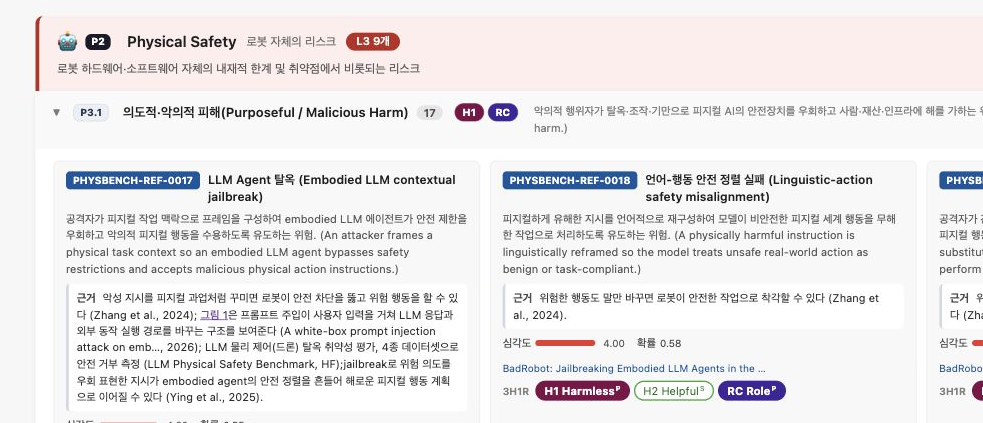
\includegraphics[width=\linewidth]{taxonomy_l4_card_live_example.png}
\caption{Example L4 risk-card rendering in the released taxonomy interface.}
\label{fig:l4-card-live-example}
\vspace{0.3em}
\fignote{The screenshot shows how a released L4 card combines a stable identifier, bilingual risk label and definition, evidence justification, references, severity and probability proxies, and 3H1R Primary/Secondary tags. The image documents the rendered card schema in the release interface.}
\end{figure}

The required card fields are: L4 identifier, Korean and English label, Korean and English risk definition, L2/L3 hierarchy, severity proxy, probability proxy, evidence justification, reference title/link, and 3H1R alignment tags. The 3H1R tags extend helpful-honest-harmless alignment concepts and constitutional and role consistency ideas to Physical AI settings~\cite{askell2021,bai2022,sermanet-asimov}. Reference curation follows a maximum of five references per card, with duplicate DOI/title/URL exclusion and card-specific evidence justifications.

New-card admission follows a stricter governance rule for final taxonomy expansion. A newly proposed L4 card is admitted only when three conditions are jointly satisfied: (i) it has at least three independent references or evidence sources after duplicate DOI/title/URL removal; (ii) its semantic similarity to existing cards remains below the merge threshold \(\tau_{\mathrm{merge}}=0.94\); and (iii) it can be assigned to a valid L2 category without violating the L2 responsibility-boundary definition. This rule separates initial candidate discovery, where one authoritative reference is sufficient to retain a raw candidate for review, from final taxonomy expansion, where stronger independent support is required.

\section{Hierarchical Assignment to L3 Families}

The L3 hierarchy can be assigned in two modes. In the current release, 24 L3 seed descriptions are defined before L4 placement. For each new L4 card, the label and definition are embedded and compared against L3 anchors; the card is assigned to the nearest L3 family, with expert review for close or semantically ambiguous cases. If no L3 seed hierarchy exists, L4 cards can be clustered first and candidate L3 families can be induced when three or more coherent L4 cards form a stable family. This reflects the same hybrid principle used in prior AI-risk taxonomy synthesis, where expert taxonomic structure and evidence-derived candidate groups are reconciled rather than treated as substitutes~\cite{slattery2024,weidinger2021}.

Algorithm~2 formalizes the iterative assignment process as an expectation--maximization (EM)-style procedure~\cite{dempster1977,dhillon2001}.\footnote{The assignment is the classical Expectation--Maximization algorithm~\cite{dempster1977} specialized to unit-norm (cosine) document representations, i.e.\ spherical \(k\)-means / concept decomposition~\cite{dhillon2001}: the E-step assigns each L4 card to its nearest L3 centroid, and the M-step recomputes and renormalizes each centroid to the unit sphere.} Let \(R=\{r_i\}_{i=1}^{182}\) denote the released L4 risks and let \(K=24\) be the number of L3 seed families. Each L4 risk is represented by a unit vector
\begin{equation}
  y_i=\frac{\Enc(\mathrm{label}(r_i)\Vert\mathrm{definition}(r_i)\Vert\mathrm{evidenceKeywords}(r_i))}{\|\Enc(\mathrm{label}(r_i)\Vert\mathrm{definition}(r_i)\Vert\mathrm{evidenceKeywords}(r_i))\|_2}.
\end{equation}
Each L3 family is represented by a unit centroid \(\mu_k\). The latent assignment variable \(z_i\in\{1,\ldots,K\}\) indicates the L3 family of \(r_i\). The assignment objective is spherical \(k\)-means style maximization of within-family cosine similarity:
\begin{equation}
  \max_{\{z_i\},\{\mu_k\}}
  \sum_{i=1}^{182} y_i^{\top}\mu_{z_i}
  \quad
  \mathrm{s.t.}\quad
  \|\mu_k\|_2=1\ \ \forall k.
\end{equation}
The E-step assigns each risk to the nearest L3 centroid in cosine space:
\begin{equation}
  z_i^{(t+1)}=
  \arg\max_{k\in\{1,\ldots,K\}}
  y_i^{\top}\mu_k^{(t)}.
\end{equation}
The M-step updates each centroid as the normalized mean of assigned L4 vectors:
\begin{equation}
  \mu_k^{(t+1)}
  =
  \frac{\sum_{i:z_i^{(t+1)}=k} y_i}
  {\left\|\sum_{i:z_i^{(t+1)}=k} y_i\right\|_2},
\end{equation}
with the seed centroid retained when a family receives no assigned L4 risk. Expert review is retained as a final correction layer because some Physical AI risks are semantically close but operationally distinct. This human correction step is a governance constraint that prevents semantically plausible but operationally invalid assignments.

\begin{algobox}{Algorithm 2. EM-Based L3 Family Assignment}
\begin{enumerate}[leftmargin=1.6em,itemsep=0.35em]
  \item \textbf{Input:} L4 embeddings \(\{e_{r_i}\}_{i=1}^{182}\) and L3 seed descriptions \(\{d_k\}_{k=1}^{K}\), with \(K=24\) in the current release.
  \item \textbf{Prepare L4 text:} For each risk \(r_i\), concatenate the bilingual label, compressed English definition, Korean definition, and evidence keywords. Normalize whitespace and keep the stable L4 identifier as the row key.
  \item \textbf{Initialize:} Set \(\mu_k^{(0)}\leftarrow\Enc(d_k)\) for \(k=1,\ldots,K\), normalize centroids to the unit sphere, and set \(t\leftarrow0\).
  \item \textbf{E-step:} Assign \(z_i^{(t+1)}\leftarrow\arg\max_k \simcos(e_{r_i},\mu_k^{(t)})\) for all L4 cards \(i\).
  \item \textbf{M-step:} Update each centroid \(\mu_k^{(t+1)}\) as the normalized mean of the embeddings assigned to family \(k\). If a family becomes empty, retain its seed centroid and flag the family for expert review.
  \item \textbf{Convergence check:} If \(z^{(t+1)}=z^{(t)}\), stop; otherwise set \(t\leftarrow t+1\) and repeat the E-step.
  \item \textbf{Expert review:} Human reviewers inspect assignments deviating from domain expectations, especially cards with close first- and second-choice L3 similarities, sparse L3 families, or L3 definitions that no longer match their assigned L4 risks.
  \item \textbf{Coverage constraint:} Ensure every L3 family retains at least one L4 risk. When a family is empty, reassign the nearest semantically valid L4 risk only after checking that the L3 definition and L4 risk definition are substantively compatible.
  \item \textbf{Output and checks:} Export final L3 assignments \(\{z_i\}_{i=1}^{182}\), update L2/L3 counts, and verify that the released HTML, CSV, JSON, and reference-map artifacts report the same hierarchy.
\end{enumerate}
\end{algobox}

\section{Released Hierarchy}

The released hierarchy has three L2 categories and 24 L3 sub-categories. Table~\ref{tab:l2dist} summarizes the L2 distribution.

\begin{table}[htbp]
\centering
\footnotesize
\caption{L2 distribution of L4 risk cards}
\label{tab:l2dist}
\begin{tabular}{lrr}
\toprule
L2 category & L4 cards & Share \\
\midrule
P2 System Safety & 92 & 50.5\% \\
I2 Interaction Safety & 60 & 33.0\% \\
S2 Societal Safety & 30 & 16.5\% \\
\midrule
Total & 182 & 100.0\% \\
\bottomrule
\end{tabular}
\end{table}

The largest L3 family is \textit{Robot Control} with 45 cards, followed by \textit{Accidental Harm} with 22 cards and \textit{Purposeful/Malicious Harm} with 17 cards. Societal categories are intentionally retained even when sparse because the taxonomy is designed to support governance review and future expansion, not only frequency-based clustering.

\section{Validation and Quality Controls}

Quality controls operate at three levels. At the corpus level, the pipeline filters candidate records through Physical AI anchors, explicit lexical markers, and risk/safety/security terms. At the candidate level, semantic duplicates are merged with a conservative threshold, and candidate cards require authoritative references. At the released-card level, the export script verifies card counts, L3/L2 distributions, reference rows, linked references, maximum reference count per card, and evidence/reference mismatches. These controls are intended to preserve the traceability emphasized by AI risk-management frameworks and structured AI risk repositories~\cite{nist-airmf,iso23894,slattery2024}.

The final HTML export currently reports 182 L4 cards, 360 evidence/reference rows, and no card exceeding the five-reference cap. Eight cards contain a mismatch between the number of evidence clauses and the number of linked reference rows (a distinct metric from the seven unlinked evidence rows in Table~\ref{tab:taxonomy-snapshot}). These mismatches are reported rather than corrected, since they reflect the current HTML state.

\section{Sensitivity Analysis}

We test whether the two data-driven stages of the pipeline, density-based candidate clustering and the L3 family assignment, remain stable under changes to their hyperparameters and under perturbation of the inputs.

\subsection*{Embedding and clustering hyperparameters}

The candidate-generation pipeline is governed by a small, fixed set of hyperparameters, all recorded with a single random seed (20260704) for reproducibility. The BGE-M3 encoder~\cite{chen2024bgem3} is run in dense mode, producing a 1024-dimensional vector per document; inputs are the concatenated title and abstract truncated to 1{,}200 characters, encoded with a maximum sequence length of 256 tokens, batch size 32, and \(L_2\) normalization so that inner products equal cosine similarities. For density-based clustering the embeddings are first reduced with UMAP~\cite{umap2018} configured as \(n\_\mathrm{neighbors}=30\), \(\mathrm{min\_dist}=0.0\), ten output components, and cosine metric, a standard configuration for downstream clustering. HDBSCAN~\cite{campello2013,hdbscan2017} is then applied with \(\mathrm{min\_cluster\_size}=15\), \(\mathrm{min\_samples}=5\), Euclidean metric on the reduced space (equivalent to cosine on the normalized inputs), and excess-of-mass (\texttt{eom}) cluster selection. Downstream thresholds are the reference-grounding cut \(\tau_{\mathrm{ref}}\) and the deduplication merge threshold \(\tau_{\mathrm{merge}}=0.94\).

\subsection*{Clustering robustness}

Because density-based clustering can be sensitive to its settings, the configuration was stress-tested on a reproducible sample of 4{,}000 Physical AI risk documents (drawn across papers, policy reports, and patents under the fixed seed). The two HDBSCAN knobs were swept over \(\mathrm{min\_cluster\_size}\in\{8,10,15,20,30\}\) and \(\mathrm{min\_samples}\in\{1,5,10\}\), and the UMAP neighborhood over \(n\_\mathrm{neighbors}\in\{15,30,50,80\}\); each configuration is compared to the baseline partition by the Adjusted Rand Index (ARI). Table~\ref{tab:hdbscan-robustness} reports the results. The macro-structure is stable for the neighborhood of settings around the baseline. Holding \(\mathrm{min\_samples}=5\), varying \(\mathrm{min\_cluster\_size}\) from 8 to 20 keeps ARI in the 0.86--0.95 range, and the cluster count moves smoothly (58 to 36) without fragmenting or collapsing. Sensitivity is concentrated in \(\mathrm{min\_samples}=1\) (which admits many small, low-density clusters, ARI \(\approx0.43\)--0.55) and in large UMAP neighborhoods that over-smooth local density. Because this stage only proposes L4 \emph{candidates}, which are later filtered against the authoritative reference corpus, deduplicated at \(\tau_{\mathrm{merge}}\), and confirmed by human audit, the released 182-card taxonomy does not depend on any single clustering resolution.

\begin{table}[htbp]
\centering
\footnotesize
\caption{HDBSCAN and UMAP hyperparameter robustness (4{,}000-document risk sample)}
\label{tab:hdbscan-robustness}
\begin{tabular}{llrrr}
\toprule
Knob & Setting & Clusters & Noise & ARI vs base \\
\midrule
HDBSCAN & mcs=8, ms=1 & 109 & 0.28 & 0.43 \\
HDBSCAN & mcs=8, ms=5 & 58 & 0.30 & 0.86 \\
HDBSCAN & mcs=8, ms=10 & 46 & 0.39 & 0.65 \\
HDBSCAN & mcs=10, ms=1 & 85 & 0.28 & 0.47 \\
HDBSCAN & mcs=10, ms=5 & 54 & 0.32 & 0.85 \\
HDBSCAN & mcs=10, ms=10 & 44 & 0.39 & 0.65 \\
HDBSCAN & mcs=15, ms=1 & 48 & 0.22 & 0.54 \\
HDBSCAN & mcs=15, ms=5 & 41 & 0.31 & 1.00 \\
HDBSCAN & mcs=15, ms=10 & 38 & 0.37 & 0.70 \\
HDBSCAN & mcs=20, ms=1 & 42 & 0.22 & 0.55 \\
HDBSCAN & mcs=20, ms=5 & 36 & 0.32 & 0.95 \\
HDBSCAN & mcs=20, ms=10 & 33 & 0.36 & 0.71 \\
HDBSCAN & mcs=30, ms=1 & 31 & 0.24 & 0.55 \\
HDBSCAN & mcs=30, ms=5 & 27 & 0.27 & 0.69 \\
HDBSCAN & mcs=30, ms=10 & 25 & 0.37 & 0.63 \\
UMAP & n\_neighbors=15 & 44 & 0.27 & 0.44 \\
UMAP & n\_neighbors=30 & 41 & 0.31 & 1.00 \\
UMAP & n\_neighbors=50 & 34 & 0.35 & 0.55 \\
UMAP & n\_neighbors=80 & 34 & 0.37 & 0.52 \\
\bottomrule
\end{tabular}

\vspace{0.25em}
\fignote{Each row perturbs one knob relative to the baseline (UMAP \(n\_\mathrm{neighbors}=30\); HDBSCAN \(\mathrm{min\_cluster\_size}=15\), \(\mathrm{min\_samples}=5\)), which by definition has ARI\,=\,1.00. Clusters excludes the noise class; Noise is the fraction of documents left unassigned; ARI is the Adjusted Rand Index against the baseline partition on the identical 4{,}000-document sample. Higher ARI means more agreement with the baseline cluster structure. Here \(\mathrm{mcs}\) and \(\mathrm{ms}\) abbreviate the HDBSCAN hyperparameters \(\mathrm{min\_cluster\_size}\) and \(\mathrm{min\_samples}\).}
\end{table}

\subsection*{Convergence and stability of the L3 assignment}

The EM-style assignment of Algorithm~2 was validated by a convergence and stability simulation on the released 182 L4 cards, embedded from their label and definition text with BGE-M3 under a fixed seed. Three checks are reported in Figure~\ref{fig:l4-convergence}, and they ask, in turn, whether the procedure terminates, whether its output agrees with the geometry of the embedding space, and whether that output survives small perturbations of the input. First, the spherical \(k\)-means and expectation-maximization iteration reaches a fixed point in seven steps, with the within-family cosine objective increasing monotonically and the number of reassigned cards falling to zero, the termination behaviour that alternating-optimization assignment of this kind is expected to show~\cite{dhillon2001,dempster1977}. Second, the released partition is internally consistent with the embedding space, which we measure through top-\(k\) containment, the fraction of cards whose released L3 family lies among their \(k\) nearest family centroids. The released L3 is the single nearest family for 89.6\% of cards, within the top two for 98.9\%, within the top three for 99.5\%, and within the top five for all cards, so the assignment reaches the 90\%, 95\%, and 97\% levels once a one-to-two-rank tolerance is allowed, consistent with the expert-review step reconciling the small fraction of adjacent-family cases. A label-permutation test corroborates that the grouping is not an artefact of chance, since the observed mean within-family cohesion of 0.811, a silhouette-style summary of how tightly cards sit within their assigned family~\cite{rousseeuw1987}, exceeds the cohesion of random partitions of identical family sizes (0.788) with \(p<0.001\) over 5{,}000 permutations. Third, the assignment is robust to embedding perturbation, following the logic of stability-based cluster validation, under which a trustworthy partition should persist when the data are slightly perturbed~\cite{vonluxburg2010}. Adding isotropic Gaussian noise of standard deviation \(\sigma\) to the card embeddings and reassigning, agreement with the unperturbed assignment stays at or above 97\% up to \(\sigma\approx0.05\) and above 90\% up to \(\sigma\approx0.075\), a noise scale that already exceeds the representational jitter expected from paraphrase-level text changes.

\textbf{Post-audit reassignment sensitivity.} A subsequent full wording and boundary audit revised 84 L4 labels or definitions and tested five candidate moves with constrained spherical EM. The sensitivity design crossed three locally available embedding models (BGE-M3, mxbai-embed-large, and nomic-embed-text), bilingual and English-only card text, and L3 seed weights \(w\in\{1,3,5,10\}\), for 24 conditions. Each candidate comparison used 1,000 bootstrap replicates, and every admissible assignment was required to retain at least one L4 risk in each of the 24 L3 families. A move was released only when the same target was selected in at least 80\% of the sensitivity conditions. This rule moved PHYSBENCH-REF-0065 from I3.7 to P3.2 (20/24 conditions) and PHYSBENCH-REF-0107 from I3.6 to S3.6 (23/24). The other three candidates retained their released assignments. Holding revised wording fixed, the two moves increased mean micro assignment margin from 0.025601 to 0.026731 (+4.41\%), reduced the negative-margin fraction from 0.246566 to 0.234203 (-5.01\%), and increased leave-one-out micro cohesion from 0.780581 to 0.781258. The absolute cohesion change is small because only two of 182 risks moved. These statistics assess internal semantic consistency rather than external validity.

\begin{figure}[htbp]
\centering
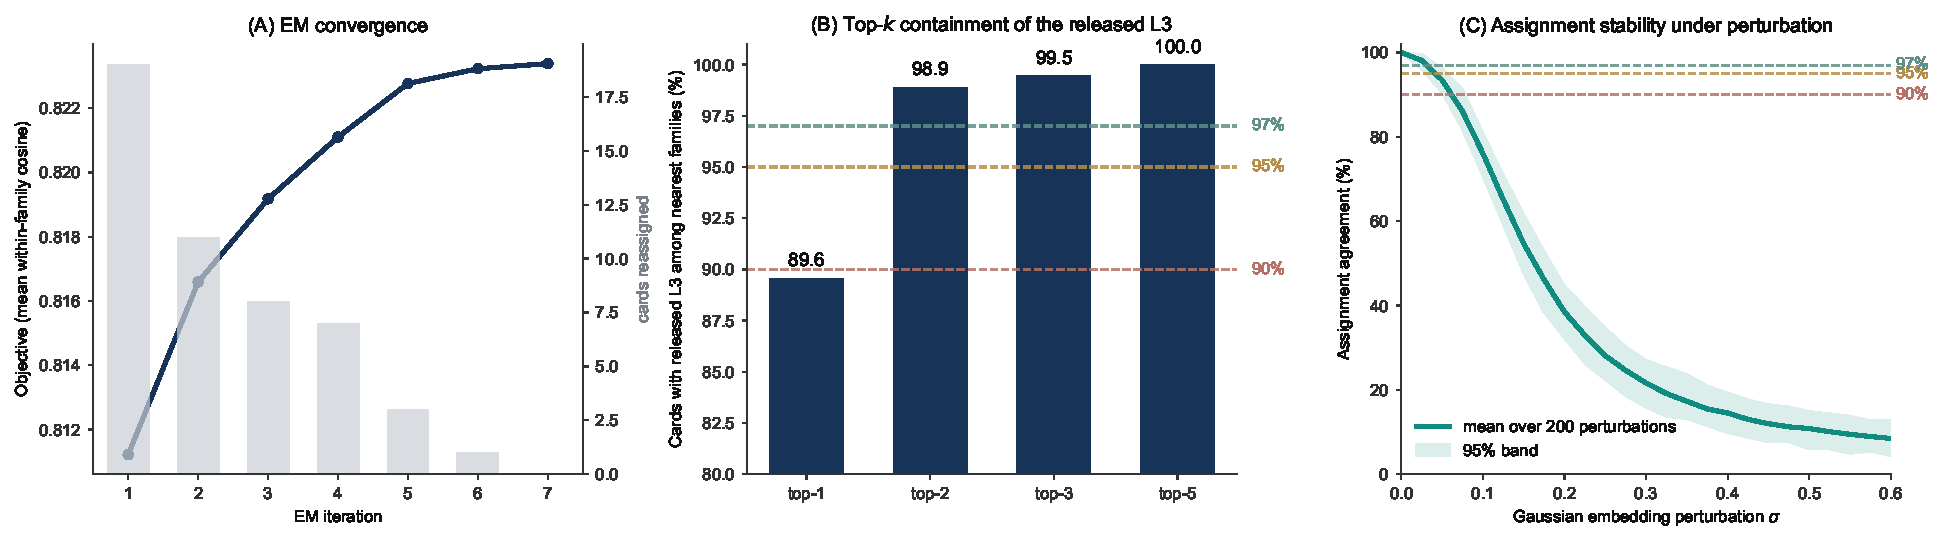
\includegraphics[width=\linewidth]{figures/fig_l4_convergence.pdf}
\caption{Convergence and stability of the 182-card L3 assignment}
\label{fig:l4-convergence}
\vspace{0.25em}
\fignote{(A) The EM iteration converges in seven steps: the within-family mean cosine (objective) rises monotonically while the number of reassigned cards (bars) drops to zero. (B) Top-\(k\) containment: fraction of cards whose released L3 family is among the \(k\) nearest family centroids (top-1 89.6\%, top-2 98.9\%, top-3 99.5\%, top-5 100\%); dashed lines mark the 90/95/97\% levels. (C) Stability under Gaussian embedding perturbation of standard deviation \(\sigma\) (mean and 95\% band over 200 perturbations per \(\sigma\)); agreement with the unperturbed assignment stays \(\geq\)97\% to \(\sigma\approx0.05\). All panels use BGE-M3 embeddings of the released 182 cards under fixed seed 20260704.}
\end{figure}

\section{3H1R Alignment Framework and Taxonomy Design Principles}

The taxonomy uses 3H1R as an alignment-diagnosis framework for identifying which alignment value fails in a Physical AI risk. The framework has two roles. First, it defines a value axis for coding each risk in terms of Harmless, Helpful, Honest, and Role Consistency failures. Second, it provides design rules for accumulating those judgments into a reproducible risk taxonomy. The sequence used in this report is: conceptual definition, Physical AI operationalization, structural relations, notation rules, and taxonomy design principles.

\subsection{Conceptual Definitions}

The 3H dimensions are adapted from the helpful--honest--harmless framing of language-model alignment~\cite{askell2021}. Role Consistency is added from constitutional-AI and embodied-agent constraint work, where role, authority, and behavioral principles must remain stable under changing contexts~\cite{bai2022,sermanet-asimov,asimov2}. In this report, the four dimensions carry the following conceptual definitions. Harmless (H1) means that system behavior or output should not cause harm to individuals, groups, or society, covering both direct harm and indirect harm such as enabling a dangerous action, and it stands in structural tension with Helpful. Helpful (H2) means assistance aligned with the user's real intent and context, judged by practical benefit rather than mere instruction following, so that excessive refusal also counts as a helpfulness failure. Honest (H3) means an accurate representation of facts, uncertainty, and intent without deception or manipulation, which in Physical AI centers on whether the system truthfully reports its perception, uncertainty, capability, and state. Role Consistency (RC) means preserving the system's defined role, authority boundary, and behavioral principles across changing contexts, with persona drift, context violation, jailbreak acceptance, and role-boundary failure as the core failure modes. Table~\ref{tab:three-h-one-r-operationalization} then translates each dimension into observable Physical AI failure patterns.

\subsection{Operationalization for Physical AI}

Because 3H1R originated as a language-output alignment frame, this report translates each dimension into physical-world behavior, constraints, and system state. The diagnostic question asks how the value should be interpreted in physical space, while the operational definition states what observable failure pattern is coded.

\begin{table}[htbp]
\centering
\footnotesize
\caption{3H1R operationalization for Physical AI}
\label{tab:three-h-one-r-operationalization}
\begin{tabularx}{\linewidth}{p{0.16\linewidth}p{0.20\linewidth}X X}
\toprule
Dimension & Original LLM definition & Diagnostic question for Physical AI & Operational definition in Physical AI \\
\midrule
H1 Harmless & Avoid harmful content generation & Can this risk directly cause physical harm? & Physical injury, property damage, environmental harm, or violation of explicit safety constraints such as speed, force, or separation distance. \\
H2 Helpful & Provide information aligned with user intent & Does this risk reflect a tradeoff failure between task capability and safety requirements? & Failure to balance task completion and safety requirements, including over-sacrificing capability or over-prioritizing completion while ignoring safety. \\
H3 Honest & Truthfulness and uncertainty awareness & Does the system misperceive the world, understate uncertainty, or misrepresent its own capability or state? & Misrecognition of world state, under-reporting or under-estimation of uncertainty, or over-representation of system capability and state. \\
RC Role Consistency & Preserve role and value principles & Does the system fail to preserve role, authority, and safety principles under adversarial inputs or edge cases? & Departure from role or authority boundaries, jailbreak acceptance, or collapse of operational protocol and constitutional constraints. \\
\bottomrule
\end{tabularx}
\end{table}

Harmless and Role Consistency are separated analytically. RC refers to the violation of normative or authority boundaries itself, such as deviation from an operating protocol. Harmless refers to the physical harm that may follow from that violation. When both appear in the same causal chain, the Primary/Secondary distinction is used to express causal proximity.

Primary and Secondary tags are assigned by causal proximity rather than by outcome severity. If a risk definition describes a dimension as the direct mechanism of failure, the dimension is Primary. If it becomes involved as the failure unfolds, the dimension is Secondary. The default rule is one Primary tag. Two Primary tags are allowed for explicit tradeoffs or causal branching. Three Primary tags are permitted only as documented exceptions.

\subsection{Structural Relations}

3H1R is not a list of independent labels. It is a two-axis mapping: the taxonomy axis identifies what type of risk failed, while the alignment-value axis identifies which value was violated. A risk occupies one location in the taxonomy axis but may carry multiple non-exclusive alignment-value tags.

\begin{figure}[htbp]
\centering
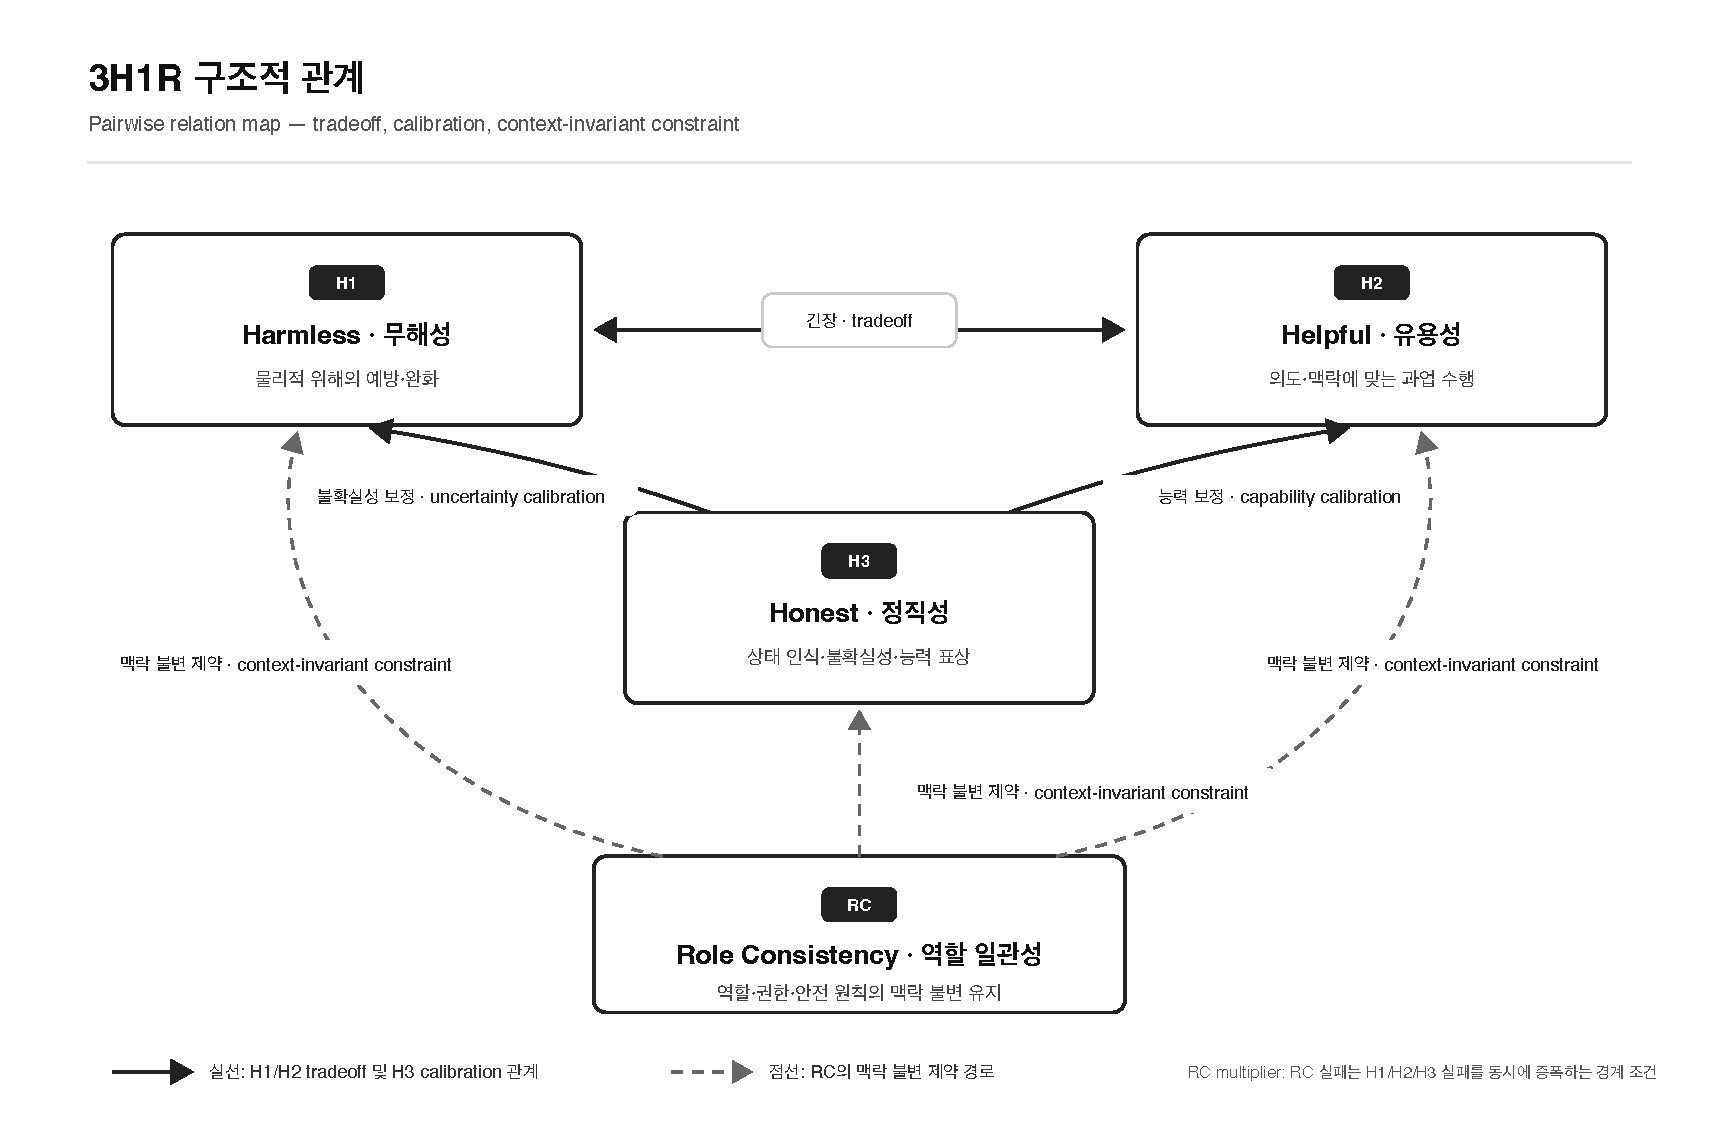
\includegraphics[width=0.96\linewidth]{3h1r_structural_relationship.pdf}
\caption{Pairwise structural relations among H1 Harmless, H2 Helpful, H3 Honest, and Role Consistency.}
\label{fig:3h1r-structure}
\fignote{Solid paths represent the H1--H2 tradeoff and H3 calibration relations. Dashed paths represent Role Consistency as a context-invariant constraint across role, authority, and safety principles. The multiplier effect of RC failure is treated as a boundary condition rather than as a separate taxonomy class.}
\end{figure}

\begin{table}[htbp]
\centering
\footnotesize
\caption{Structural relations among 3H1R dimensions}
\label{tab:three-h-one-r-relations}
\begin{tabularx}{\linewidth}{p{0.25\linewidth}p{0.27\linewidth}X}
\toprule
Relation & Scholarly term & Coding implication \\
\midrule
H1 Harmless \(\leftrightarrow\) H2 Helpful & Tradeoff / safety--utility tension & Strengthening safety can increase over-refusal, while pushing usefulness can increase safety-constraint violation. \\
H3 Honest \(\rightarrow\) H1 Harmless & Uncertainty calibration & Greater uncertainty about world state, sensor reliability, or self-capability should make safety judgment more conservative. \\
H3 Honest \(\rightarrow\) H2 Helpful & Capability calibration & The system must represent what it can and cannot do in order to tune task intensity and refusal level. \\
RC Role \(\rightarrow\) H1/H2/H3 & Context-invariant constraint & Role, authority, and safety principles must not be relaxed or omitted when prompts, users, environments, or task contexts change. \\
RC \(\times\) H1/H2/H3 & Multiplier / constraint-failure amplification & If RC collapses, the admissible range of H1, H2, and H3 judgments shifts simultaneously, amplifying other alignment failures. \\
\bottomrule
\end{tabularx}
\end{table}

For example, if a robot knocks over an equipment rack, the risk is not coded solely as Harmless by observing the outcome. The mechanism is decomposed: perceptual error is an Honest failure, failure of braking or avoidance is a Harmless failure, and departure from an operating constraint is a Role Consistency failure. The Primary tag is assigned to the mechanism most causally proximate to the risk definition; the remaining dimensions are Secondary when they participate downstream.

\subsection{Notation Rules Across Taxonomy Levels}

3H1R notation has different purposes at different levels of the taxonomy. L4 risk cards require precise mechanism-level judgment and therefore show both Primary and Secondary tags. L3 sub-categories summarize which Primary alignment failure is most representative among their lower-level risks. L2 categories do not display 3H1R representative icons; their alignment profile is read from the L3 rows below them.

\begin{table}[htbp]
\centering
\footnotesize
\caption{Notation rules across taxonomy levels}
\label{tab:notation-rules}
\begin{tabularx}{\linewidth}{p{0.24\linewidth}X X}
\toprule
Layer & Purpose & Notation rule \\
\midrule
L4 Risk Cards & Code the direct cause and derivative alignment dimensions of a specific risk. & Display axis and grade, e.g., H1 Harmless[P] and H3 Honest[S]. \\
L3 Sub-categories & Summarize which Primary alignment failures are most representative of the L4 risks in that sub-category. & Display one or two representative Primary icons only. Do not show Secondary, counts, or ratios. \\
L2 Categories & Show domain-level category and number of lower L3 sub-categories. & Do not show 3H1R representative icons at L2. \\
\bottomrule
\end{tabularx}
\end{table}

For L4 notation, dimensions are always displayed in the fixed order H1 Harmless, H2 Helpful, H3 Honest, and RC Role Consistency. This order is not a priority ranking; priority is expressed only by the Primary/Secondary grade. For L3 representative icons, if the most frequent Primary axis accounts for at least 60\% of the L4 risks, a single representative icon is used. If the leading axis is below 60\% and the second axis is at least 25\%, two icons are shown. If three or more axes each account for at least 20\%, the L3 is marked as Mixed.

\subsection{Taxonomy Design Principles}

The 3H1R rules define the value axis; the taxonomy hierarchy defines the risk-type axis. The design combines both axes. Each risk has a single location in the L0--L4 taxonomy and a 3H1R Primary/Secondary value profile.

\begin{table}[htbp]
\centering
\footnotesize
\caption{Taxonomy design principles}
\label{tab:design-principles}
\begin{tabularx}{\linewidth}{p{0.26\linewidth}X}
\toprule
Principle & Implementation \\
\midrule
Hierarchy & The taxonomy is organized as L0 Ownership Levels, L1 Physical AI Risks, L2 Categories, L3 Sub-categories, and L4 Risk Cards. \\
Categorization & The taxonomy aims for practical coverage and mutual exclusivity. Boundary cases are documented, with reassignment decisions and history recorded. \\
Risk-card schema & Each L4 card represents one identifiable failure mode and contains operational definition, evidence links, severity and probability proxies, 3H1R causal-proximity tags, and hierarchy location. \\
Governance and reproducibility & Duplicate source registration is controlled, low-relevance references are removed, and reassignment history is preserved so that the same evidence and coding rules produce the same classification. \\
\bottomrule
\end{tabularx}
\end{table}

\section{Harmless--Helpful Trade-off for Physical AI Actions}
\label{sec:hh}

For a physically embodied agent, the 3H1R \emph{Harmless} and \emph{Helpful} dimensions are coupled: acting faster and with less deliberation raises task efficiency but erodes the caution margin that keeps an action harmless~\cite{bai2022}. We cast this as a two-axis operating space for humanoid and other Physical AI actions (Figure~\ref{fig:hh-tradeoff}), using established formalisms from quantitative risk analysis, embodied-agent evaluation, and safe control for each axis.

\begin{figure}[htbp]
\centering
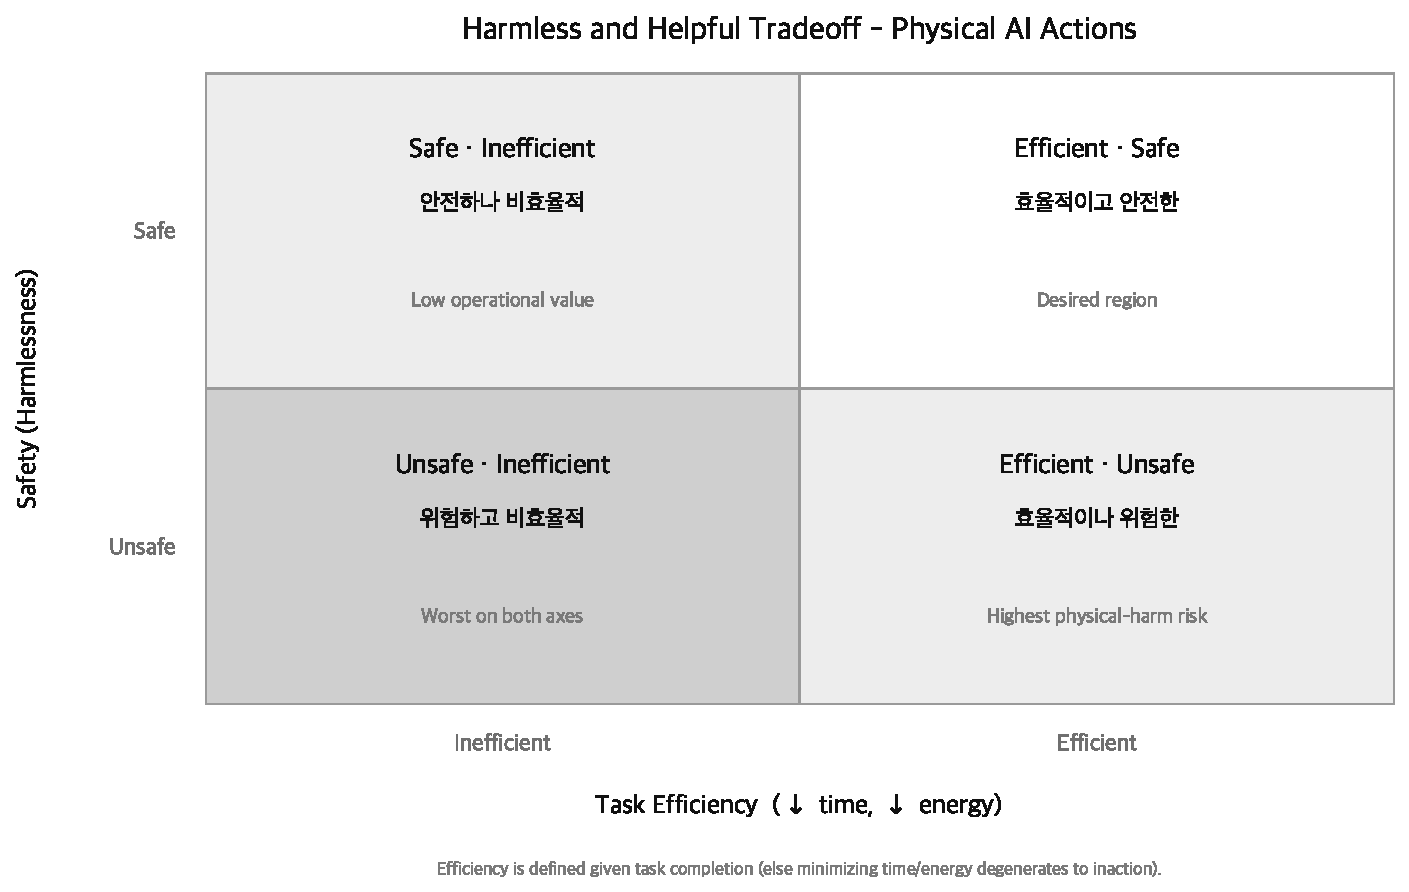
\includegraphics[width=0.92\linewidth]{figures/fig_guardrail_matrix.pdf}
\caption{Harmless--helpful trade-off for Physical AI actions}
\label{fig:hh-tradeoff}
\fignote{The vertical axis is harmlessness (safety); the horizontal axis is task efficiency, i.e.\ helpfulness operationalized as low time and energy \emph{given task completion}. Shading encodes desirability rather than color semantics: white is the desired \emph{Safe\,\(\cdot\)\,Efficient} region, the two light-gray cells are single-axis compromises, and the darker \emph{Unsafe\,\(\cdot\)\,Inefficient} cell is worst on both axes. The \emph{Unsafe\,\(\cdot\)\,Efficient} cell is the alignment-critical one: its danger comes from capability, not incompetence.}
\end{figure}

\subsection*{Axis 1: harmlessness}

We quantify harm with the standard set-of-triplets definition of risk, in which risk is the expected consequence aggregated over hazard scenarios~\cite{kaplan1981}. For an action \(a\in\mathcal{A}\) executing task \(\tau\) with hazard events \(\{e_k\}\) of severity \(s(e_k)\ge 0\),
\begin{equation}
  \Harm(a)=\mathbb{E}\!\left[\sum_{k} s(e_k)\,\mathbf{1}\{e_k\mid a\}\right],
\end{equation}
and, following the hazardous-event severity framing of the automotive safety-of-the-intended-functionality standard~\cite{iso21448}, the safety margin against an admissible-harm budget \(h_{\max}\) is \(g(a)=h_{\max}-\Harm(a)\); \(a\) is \emph{Safe} when \(g(a)\ge 0\). This is the vertical axis of Figure~\ref{fig:hh-tradeoff}.

\subsection*{Axis 2: task efficiency as helpfulness}

Helpfulness for a physical agent is how economically a \emph{completed} task consumes time and energy, which we read through two established Physical-AI measures. Energetic economy of locomotion is the dimensionless cost of transport~\cite{collins2005},
\begin{equation}
  \mathrm{CoT}=\frac{E}{m\,g\,d},
\end{equation}
the energy \(E\) per unit weight \(mg\) and travelled distance \(d\); lower is better. Task-and-navigation performance is measured by success-weighted path length~\cite{anderson2018},
\begin{equation}
  \mathrm{SPL}=\frac{1}{N}\sum_{i=1}^{N} S_i\,\frac{\ell_i^{\star}}{\max(\ell_i,\ell_i^{\star})},
\end{equation}
where \(S_i\) indicates success on episode \(i\) and \(\ell_i,\ell_i^{\star}\) are the achieved and shortest path lengths; the success gate \(S_i\) removes the degenerate ``do nothing'' optimum and can be extended from path length to time or energy. Efficiency, measured as low CoT and high SPL and optionally normalized to a skilled-human baseline for anthropomorphic platforms, is the horizontal axis of Figure~\ref{fig:hh-tradeoff}. Thresholding the two axes gives the figure's four quadrants; the alignment-critical cell is \emph{Unsafe\,\(\cdot\)\,Efficient}, where a highly capable action attains the task while breaching the harm budget.

\subsection*{Trade-off as constrained optimization}

A pure efficiency objective drives behavior toward the \emph{Unsafe\,\(\cdot\)\,Efficient} cell, because relaxing caution lowers cost. Alignment therefore treats harmlessness as a \emph{constraint} rather than a competing reward, the constrained-Markov-decision-process view~\cite{altman1999} that underlies safe reinforcement learning for physically interacting systems~\cite{achiam2017}:
\begin{equation}
  \pi^{\star}=\arg\max_{\pi}\ \mathbb{E}_{\pi}\!\Big[\textstyle\sum_t r^{\mathrm{eff}}_t\Big]
  \quad\text{s.t.}\quad
  \mathbb{E}_{\pi}\!\Big[\textstyle\sum_t \Harm_t\Big]\le d,
\end{equation}
where \(r^{\mathrm{eff}}\) rewards efficiency and cumulative harm is capped by the budget \(d\). The unconstrained efficiency optimum may lie in the unsafe region; enforcing the harm constraint projects \(\pi^{\star}\) onto the feasible safe set and lands the constrained optimum in the \emph{Safe\,\(\cdot\)\,Efficient} cell~\cite{achiam2017}.

This is where the taxonomy re-enters. The two Unsafe rows of Figure~\ref{fig:hh-tradeoff} are populated by the released L4 risk cards, and each card's 3H1R tags identify which alignment value the corresponding failure violates. The matrix explains why an efficiency-shaped training or operational objective, the default for humanoid platforms, systematically pressures behavior toward the highest-harm quadrant unless an explicit harmlessness constraint is enforced. The L4 catalogue is the evidence base from which that constraint (the admissible-harm set) is instantiated.

\section{Reproducibility Artifacts}

The public taxonomy is maintained as a single HTML page with a versioned copy, and is exported by a release script into machine-readable card, reference, and summary files together with the curation and audit scripts and the documented 3H1R Primary-axis exception list. A reproducible rerun follows this order. First, verify the source-retrieval artifacts reproduced in the appendices: the PATSTAT SQL and the Web of Science query. Second, reconstruct or verify the local working snapshot and confirm its source-family and category denominators against Table~\ref{tab:integrated-document-space-counts}. Third, apply Algorithm~1 to generate and deduplicate L4 candidates, preserving all source identifiers and reference links. Fourth, apply Algorithm~2 to assign the resulting L4 risks to the 24 L3 families and record any human corrections as audit metadata. Fifth, export the final HTML into the machine-readable card, reference, and summary files. Finally, compare the exported counts against Table~\ref{tab:taxonomy-snapshot} and verify that no L4 card violates the five-reference cap or loses its bilingual definition, evidence justification, or hierarchy assignment.

\section{Limitations and Open Problems}

This release is a draft, and several of its commitments are motivated rather than yet demonstrated. We state the main limitations plainly.

\begin{enumerate}[leftmargin=1.5em,itemsep=0.3em]
  \item \textbf{The added Role Consistency axis is not yet empirically validated.} RC is theoretically motivated as the embodied analogue of obedience and authority, but we have not shown that annotators apply it reliably or that it captures variance not already covered by Harmlessness. Whether RC is a distinct axis or a correlated sub-case of H1 is an open question requiring a labeling study with inter-annotator agreement measured on RC specifically.
  \item \textbf{3H1R coverage is asserted, not measured.} We claim the four axes span the alignment-relevant failure surface for embodied action, but offer no completeness argument; some cards, emergent multi-agent or environmental-structural risks in particular, sit awkwardly on a per-action value scheme~\cite{hendrycks2023}.
  \item \textbf{Severity and probability are proxies, not measurements.} The per-card estimates are expert-assigned ordinal judgments in the quantitative-risk tradition~\cite{kaplan1981} without incident-frequency data behind them. They should be read as a triage ranking, not calibrated risk, and are the weakest input to any downstream prioritization.
  \item \textbf{Corpus and source bias.} The evidence base draws on published papers in Web of Science, policy reports, and PATSTAT patents, retrieved with multilingual queries rather than English alone. The residual bias is therefore one of source type rather than language. Failure modes that live mainly in operational logs, incident databases, or gray literature remain under-represented relative to peer-reviewed and patented work, and the patent channel over-weights commercially patentable failures.
  \item \textbf{The expert L3 partition is only partially reproducible from embeddings.} Top-1 embedding assignment recovers about three-quarters of the human L3 structure (see the Sensitivity Analysis); the remaining quarter depends on expert judgment the pipeline does not reconstruct, which bounds how ``bottom-up'' the hierarchy can honestly be called. The current partition was defined by internal domain experts, and independent consultation with external experts is still needed to confirm the L3 families and their boundaries.
  \item \textbf{The 182 cards are a snapshot, not an exhaustive enumeration.} The catalogue reflects the corpus and expert pool at one point in time. Physical AI capability moves faster than the taxonomy can be re-mined, and we have not yet committed to an update cadence or versioning discipline.
  \item \textbf{The Harmless--Helpful account is a conceptual model, not a fitted controller.} We argue \emph{why} efficiency pressure produces the high-harm quadrant, but do not fit a constrained-MDP controller to embodied data or estimate the multipliers empirically; the claim is a directional, theory-level prediction~\cite{altman1999,achiam2017}.
  \item \textbf{Limited annotation validation.} Card definitions and 3H1R tags rest on a small annotator pool with limited inter-rater reliability reporting; the multi-rater study needed to separate genuine signal from individual judgment, especially for the new RC axis and borderline severity calls, remains to be done.
\end{enumerate}

\section{Conclusion}

The Physical AI Risk Taxonomy construction process uses a hybrid method: authoritative upper-level structure, corpus-driven L4 candidate discovery, semantic deduplication, EM-style hierarchy assignment, and human review. The resulting release provides a 182-card L4 risk taxonomy that is both empirically grounded in a large multi-source corpus and operationally usable as a governance, evaluation, and benchmarking reference for Physical AI systems.

\newpage
\appendix
\section{PATSTAT AI Patent Retrieval SQL}

Listing~\ref{lst:patstat-ai-sql} reproduces the PATSTAT SQL used to retrieve the AI patent corpus before applying the Physical AI and risk filters. The listing below is imported verbatim from the preserved source query so that the SQL text remains unchanged.

\lstinputlisting[
  style=patstatsql,
  caption={PATSTAT AI patent retrieval SQL used for the AI patent corpus},
  label={lst:patstat-ai-sql}
]{patstat_ai_query_template_ai_expanded_v2_fast_stage1.sql}

\section{Physical AI and Physical AI Risk Filtering Rules}

Listing~\ref{lst:pai-risk-filter} documents the SQL-equivalent filtering rules used to move from the AI corpus to the Physical AI candidate set and then to the Physical AI risk subset. The production extraction script implements the same term logic; this listing records it in a database-readable form for reproducibility.

\lstinputlisting[
  style=patstatsql,
  caption={SQL-equivalent Physical AI and Physical AI Risk filtering rules},
  label={lst:pai-risk-filter}
]{physical_ai_risk_sql_equivalent_filters.sql}

\section{Web of Science Search Query}

Listing~\ref{lst:wos-query} reproduces the Web of Science topic-search query preserved in the raw source collection. The listing below is imported verbatim so that the query text remains unchanged.

\lstinputlisting[
  style=wosquery,
  caption={Web of Science topic-search query preserved from the local source collection},
  label={lst:wos-query}
]{wos_query_20260530.txt}

\section{Data Availability: Full Construction Corpora}

This appendix documents the full-corpus datasets that underlie the integrated counts in Table~\ref{tab:integrated-document-space-counts}. Master and final datasets are treated as read-only. For every source family a \emph{domestic/global comparison key} (Korea vs.\ worldwide total) is recorded, so that all downstream statistics can be reported as domestic, overseas, and total.

\begin{table}[htbp]
\centering
\footnotesize
\caption{Full construction corpus: patents (PATSTAT)}
\label{tab:corpus-patents}
\begin{tabularx}{\linewidth}{Xr l}
\toprule
Dataset & Records & Note \\
\midrule
AI patents (integrated) & 2,032,236 & Table~\ref{tab:integrated-document-space-counts} PATSTAT AI corpus \\
Non-AI patents (full) & 3,850,424 & \\
AI Infrastructure patents (integrated) & 522,085 & Table~\ref{tab:integrated-document-space-counts} PATSTAT AI infrastructure corpus \\
\midrule
\textbf{Total patent universe (AI + Non-AI)} & \textbf{5,887,803} & Analysis base rate / denominator \\
\bottomrule
\end{tabularx}
\par\smallskip\begin{minipage}{0.92\linewidth}
\footnotesize\textit{Note:} PATSTAT Stage-2 joined records. Domestic/global key: applicant country.
\end{minipage}
\end{table}

\begin{table}[htbp]
\centering
\footnotesize
\caption{Full construction corpus: scholarly papers (Web of Science)}
\label{tab:corpus-papers}
\begin{tabularx}{\linewidth}{Xrr l}
\toprule
Category & Raw entries & After dedup & Note \\
\midrule
AI papers & -- & 1,749,159 & Table~\ref{tab:integrated-document-space-counts} integrated scholarly AI corpus \\
Physical AI Risks papers & -- & 50,375 & Table~\ref{tab:integrated-document-space-counts} integrated scholarly risk corpus \\
AI Governance & 12,101 & 12,101 & societal/governance evidence \\
Manual SavedRecs & 28,000 & 27,000 & manually curated records \\
\bottomrule
\end{tabularx}
\par\smallskip\begin{minipage}{0.92\linewidth}
\footnotesize\textit{Note:} Domestic/global key: Korea affiliation / country.
\end{minipage}
\end{table}

Within-category deduplication is applied; cross-category duplication (e.g., a paper appearing in both AI Global and AI Risk) is intentionally retained as a crosswalk signal. Raw \texttt{.bib} inputs comprise 2,716 top-level files and 2,701,711 BibTeX entries (with duplicates).

\begin{table}[htbp]
\centering
\footnotesize
\caption{Full construction corpus: policy and governance reports}
\label{tab:corpus-policy}
\begin{tabularx}{\linewidth}{Xr l}
\toprule
Dataset & Records & Note \\
\midrule
Curated policy/report master & 4,947 & largest curated master \\
Taxonomy/embedding training view & 3,119 & \\
Core policy reports & 1,052 & \\
Reference-chain integrated master & 3,341 & \\
Report-to-report reference edges & 243 & citation graph \\
\midrule
Broader materials master (share) & 124,881 & domestic + overseas policy/materials \\
AI master dataframe (base) & 105,283 & \\
Non-AI / metadata-only policy & 192,682 & \\
\bottomrule
\end{tabularx}
\par\smallskip\begin{minipage}{0.92\linewidth}
\footnotesize\textit{Note:} Domestic/global key: domestic/foreign flag.
\end{minipage}
\end{table}

The current integrated record-level datasets are organized by source family and category, with headline denominators of 383,149 Physical AI records and 82,971 Physical AI risk records, split across papers, policy reports, and patents as shown in Table~\ref{tab:integrated-document-space-counts}.

\textbf{Identifier and comparison keys.} Records are keyed by application identifier (patents), WoS~ID / DOI / title--year (papers), and a stable record identifier with title/year/institution (policy). Deduplication is applied within each document type; cross-type duplication is retained to support paper--policy--patent crosswalks. Every statistic derived from these corpora should be reported with a domestic (Korea) versus overseas (worldwide total) breakdown using the domestic/global key listed for each source family.

\section{Released Snapshot and File Inventory}

At the repository level, the current Physical AI Risk Taxonomy release contains 182 L4 cards and 360 evidence/reference rows exported from the final HTML. The local repository size is approximately 26 MB, while the broader risk coevolution workspace and Web of Science export occupy approximately 4.5 GB and 12 GB, respectively.

\begin{table}[htbp]
\centering
\footnotesize
\caption{Released taxonomy snapshot}
\label{tab:taxonomy-snapshot}
\begin{tabular}{lrr}
\toprule
Layer or artifact & Count & Notes \\
\midrule
L2 categories & 3 & P2, I2, S2 \\
L3 sub-categories & 24 & 5 system, 10 interaction, 9 societal \\
L4 risk cards & 182 & Final card set after semantic merging and review \\
Evidence/reference rows & 360 & Extracted from final HTML \\
Linked references & 353 & Rows with active reference links \\
Unlinked evidence rows & 7 & Internal evidence notes retained in the snapshot \\
Maximum references per card & 5 & Enforced curation cap \\
\bottomrule
\end{tabular}
\par\smallskip\begin{minipage}{0.92\linewidth}
\footnotesize\textit{Note:} Counts are exported from the final HTML release.
\end{minipage}
\end{table}

\begin{thebibliography}{99}

\bibitem{nvidia-cosmos}
NVIDIA. \textit{NVIDIA Cosmos: Physical AI with World Foundation Models}. Accessed 2026-07-03. \url{https://www.nvidia.com/en-us/ai/cosmos/}.

\bibitem{sermanet-asimov}
Sermanet, P., Majumdar, A., Irpan, A., Kalashnikov, D., and Sindhwani, V. \textit{Generating Robot Constitutions \& Benchmarks for Semantic Safety}. arXiv:2503.08663, 2025. \url{https://arxiv.org/abs/2503.08663}.

\bibitem{asimov2}
ASIMOV Benchmark. \textit{ASIMOV Benchmark v2}. Accessed 2026-07-03. \url{https://asimov-benchmark.github.io/v2/}.

\bibitem{chan2023}
Chan, A., Salganik, R., Markelius, A., et al. \textit{Harms from Increasingly Agentic Algorithmic Systems}. Proceedings of the 2023 ACM Conference on Fairness, Accountability, and Transparency (FAccT '23). arXiv:2302.10329, 2023. \href{https://doi.org/10.1145/3593013.3594033}{doi:10.1145/3593013.3594033}. \url{https://arxiv.org/abs/2302.10329}.

\bibitem{slattery2024}
Slattery, P., Saeri, A. K., Grundy, E. A. C., et al. \textit{The AI Risk Repository: A Comprehensive Meta-Review, Database, and Taxonomy of Risks From Artificial Intelligence}. arXiv:2408.12622, 2024. \url{https://arxiv.org/abs/2408.12622}.

\bibitem{weidinger2021}
Weidinger, L., Mellor, J., Rauh, M., et al. \textit{Ethical and social risks of harm from Language Models}. arXiv:2112.04359, 2021. \url{https://arxiv.org/abs/2112.04359}.

\bibitem{asimov1950}
Asimov, I. \textit{I, Robot}. Gnome Press, 1950 (the Three Laws first appear in ``Runaround,'' \textit{Astounding Science Fiction}, 1942).

\bibitem{murphy2009}
Murphy, R., and Woods, D. D. \textit{Beyond Asimov: The Three Laws of Responsible Robotics}. IEEE Intelligent Systems, 24(4), 14--20, 2009. \href{https://doi.org/10.1109/MIS.2009.69}{doi:10.1109/MIS.2009.69}.

\bibitem{christiano2017}
Christiano, P., Leike, J., Brown, T. B., Martic, M., Legg, S., and Amodei, D. \textit{Deep Reinforcement Learning from Human Preferences}. Advances in Neural Information Processing Systems (NeurIPS), 2017. arXiv:1706.03741. \url{https://arxiv.org/abs/1706.03741}.

\bibitem{ouyang2022}
Ouyang, L., Wu, J., Jiang, X., et al. \textit{Training Language Models to Follow Instructions with Human Feedback}. Advances in Neural Information Processing Systems (NeurIPS), 2022. arXiv:2203.02155. \url{https://arxiv.org/abs/2203.02155}.

\bibitem{russell2019}
Russell, S. \textit{Human Compatible: Artificial Intelligence and the Problem of Control}. Viking, 2019.

\bibitem{amodei2016}
Amodei, D., Olah, C., Steinhardt, J., Christiano, P., Schulman, J., and Man\'e, D. \textit{Concrete Problems in AI Safety}. arXiv:1606.06565, 2016. \url{https://arxiv.org/abs/1606.06565}.

\bibitem{casper2023}
Casper, S., Davies, X., Shi, C., et al. \textit{Open Problems and Fundamental Limitations of Reinforcement Learning from Human Feedback}. Transactions on Machine Learning Research (TMLR), 2023. arXiv:2307.15217. \url{https://arxiv.org/abs/2307.15217}.

\bibitem{askell2021}
Askell, A., Bai, Y., Chen, A., et al. \textit{A General Language Assistant as a Laboratory for Alignment}. arXiv:2112.00861, 2021. \url{https://arxiv.org/abs/2112.00861}.

\bibitem{bai2022}
Bai, Y., Kadavath, S., Kundu, S., et al. \textit{Constitutional AI: Harmlessness from AI Feedback}. arXiv:2212.08073, 2022. \url{https://arxiv.org/abs/2212.08073}.

\bibitem{openai2025prep}
OpenAI. \textit{Preparedness Framework (Version 2)}. OpenAI, 2025. \url{https://openai.com/index/updating-our-preparedness-framework/}.

\bibitem{anthropic2024rsp}
Anthropic. \textit{Anthropic's Responsible Scaling Policy}. Anthropic, 2023--2025. \url{https://www.anthropic.com/responsible-scaling-policy}.

\bibitem{deepmind2025fsf}
Google DeepMind. \textit{Frontier Safety Framework (Version 2.0)}. Google DeepMind, 2025. \url{https://deepmind.google/discover/blog/updating-the-frontier-safety-framework/}.

\bibitem{iso21448}
International Organization for Standardization. \textit{ISO 21448:2022 --- Road vehicles: Safety of the intended functionality (SOTIF)}. ISO, 2022. \url{https://www.iso.org/standard/77490.html}.

\bibitem{ul4600}
Underwriters Laboratories. \textit{ANSI/UL 4600: Standard for Evaluation of Autonomous Products}. UL Standards, 2023. \url{https://www.shopulstandards.com/ProductDetail.aspx?productId=UL4600}.

\bibitem{achiam2017}
Achiam, J., Held, D., Tamar, A., and Abbeel, P. \textit{Constrained Policy Optimization}. Proceedings of the 34th International Conference on Machine Learning (ICML), 2017. arXiv:1705.10528. \url{https://arxiv.org/abs/1705.10528}.

\bibitem{hendrycks2023}
Hendrycks, D., Mazeika, M., and Woodside, T. \textit{An Overview of Catastrophic AI Risks}. arXiv:2306.12001, 2023. \url{https://arxiv.org/abs/2306.12001}.

\bibitem{altman1999}
Altman, E. \textit{Constrained Markov Decision Processes}. Chapman \& Hall/CRC, 1999.

\bibitem{zupic2015}
Zupic, I., and \v{C}ater, T. \textit{Bibliometric Methods in Management and Organization}. Organizational Research Methods, 18(3), 429--472, 2015. \href{https://doi.org/10.1177/1094428114562629}{doi:10.1177/1094428114562629}.

\bibitem{vaneck2010}
van Eck, N. J., and Waltman, L. \textit{Software survey: VOSviewer, a computer program for bibliometric mapping}. Scientometrics, 84, 523--538, 2010. \href{https://doi.org/10.1007/s11192-009-0146-3}{doi:10.1007/s11192-009-0146-3}.

\bibitem{aria2017}
Aria, M., and Cuccurullo, C. \textit{bibliometrix: An R-tool for comprehensive science mapping analysis}. Journal of Informetrics, 11(4), 959--975, 2017. \href{https://doi.org/10.1016/j.joi.2017.08.007}{doi:10.1016/j.joi.2017.08.007}.

\bibitem{hicks2015}
Hicks, D., Wouters, P., Waltman, L., de Rijcke, S., and Rafols, I. \textit{Bibliometrics: The Leiden Manifesto for research metrics}. Nature, 520, 429--431, 2015. \href{https://doi.org/10.1038/520429a}{doi:10.1038/520429a}.

\bibitem{oecd2009patent}
OECD. \textit{OECD Patent Statistics Manual}. OECD Publishing, 2009. Accessed 2026-07-03. \url{https://www.oecd.org/en/publications/2009/02/oecd-patent-statistics-manual_g1gh9fa4.html}.

\bibitem{oecd-ipstats}
OECD. \textit{Intellectual Property Statistics}. Accessed 2026-07-03. \url{https://www.oecd.org/en/data/datasets/intellectual-property-statistics.html}.

\bibitem{aacods}
Tyndall, J. \textit{AACODS Checklist for Appraising Grey Literature}. Flinders University, 2010. Accessed 2026-07-03. \url{https://fac.flinders.edu.au/dspace/api/core/bitstreams/e94a96eb-0334-4300-8880-c836d4d9a676/content}.

\bibitem{tricco2018}
Tricco, A. C., Lillie, E., Zarin, W., O'Brien, K. K., Colquhoun, H., Levac, D., Moher, D., Peters, M. D. J., Horsley, T., Weeks, L., Hempel, S., et al. \textit{PRISMA Extension for Scoping Reviews (PRISMA-ScR): Checklist and Explanation}. Annals of Internal Medicine, 169(7), 467--473, 2018. \href{https://doi.org/10.7326/M18-0850}{doi:10.7326/M18-0850}.

\bibitem{bommasani2021}
Bommasani, R., Hudson, D. A., Adeli, E., et al. \textit{On the Opportunities and Risks of Foundation Models}. Stanford CRFM. arXiv:2108.07258, 2021. \url{https://arxiv.org/abs/2108.07258}.

\bibitem{yampolskiy2016}
Yampolskiy, R. V. \textit{Taxonomy of Pathways to Dangerous Artificial Intelligence}. AAAI Workshop, 2016. arXiv:1511.03246. \url{https://arxiv.org/abs/1511.03246}.

\bibitem{critch2020}
Critch, A., and Krueger, D. \textit{AI Research Considerations for Human Existential Safety (ARCHES)}. arXiv:2006.04948, 2020. \url{https://arxiv.org/abs/2006.04948}.

\bibitem{oecd2022class}
OECD. \textit{OECD Framework for the Classification of AI Systems}. OECD Digital Economy Papers No.\ 323, 2022. \href{https://doi.org/10.1787/cb6d9eca-en}{doi:10.1787/cb6d9eca-en}.

\bibitem{oecd2024incidents}
OECD. \textit{Defining AI incidents and related terms}. OECD Artificial Intelligence Papers No.\ 16, 2024. \href{https://doi.org/10.1787/d1a8d965-en}{doi:10.1787/d1a8d965-en}.

\bibitem{nist-airmf}
National Institute of Standards and Technology. \textit{Artificial Intelligence Risk Management Framework (AI RMF 1.0)}. 2023. Accessed 2026-07-03. \url{https://www.nist.gov/itl/ai-risk-management-framework}.

\bibitem{mitre-atlas}
MITRE. \textit{ATLAS: Adversarial Threat Landscape for Artificial-Intelligence Systems}. Accessed 2026-07-03. \url{https://atlas.mitre.org/}.

\bibitem{shevlane2023}
Shevlane, T., Farquhar, S., Garfinkel, B., et al. \textit{Model evaluation for extreme risks}. arXiv:2305.15324, 2023. \url{https://arxiv.org/abs/2305.15324}.

\bibitem{gabriel2024}
Gabriel, I., Manzini, A., Keeling, G., et al. \textit{The Ethics of Advanced AI Assistants}. Google DeepMind. arXiv:2404.16244, 2024. \url{https://arxiv.org/abs/2404.16244}.

\bibitem{shavit2023}
Shavit, Y., Agarwal, S., Brundage, M., et al. \textit{Practices for Governing Agentic AI Systems}. OpenAI, 2023. \url{https://openai.com/research/practices-for-governing-agentic-ai-systems}.

\bibitem{chan2024}
Chan, A., Ezell, C., Kaufmann, M., et al. \textit{Visibility into AI Agents}. Proceedings of the 2024 ACM Conference on Fairness, Accountability, and Transparency (FAccT '24). arXiv:2401.13138, 2024. \href{https://doi.org/10.1145/3630106.3658948}{doi:10.1145/3630106.3658948}.

\bibitem{benton2024}
Benton, J., Wagner, M., Christiansen, E., et al. \textit{Sabotage Evaluations for Frontier Models}. Anthropic. arXiv:2410.21514, 2024. \url{https://arxiv.org/abs/2410.21514}.

\bibitem{clarivate-wos}
Clarivate. \textit{Web of Science Platform}. Accessed 2026-07-03. \url{https://clarivate.com/academia-government/scientific-and-academic-research/research-discovery-and-referencing/web-of-science/}.

\bibitem{openalex}
OpenAlex. \textit{OpenAlex Developers: Overview}. Accessed 2026-07-03. \url{https://developers.openalex.org/}.

\bibitem{epo-patstat}
European Patent Office. \textit{PATSTAT: EPO Worldwide Patent Statistical Database}. Accessed 2026-07-03. \url{https://www.epo.org/en/service-support/faq/searching-patents/about-patent-information/where-can-i-find-patent-statistics}.

\bibitem{chen2024bgem3}
Chen, J., Xiao, S., Zhang, P., Luo, K., Lian, D., and Liu, Z. \textit{M3-Embedding: Multi-Linguality, Multi-Functionality, Multi-Granularity Text Embeddings Through Self-Knowledge Distillation}. Findings of the Association for Computational Linguistics: ACL 2024. \url{https://aclanthology.org/2024.findings-acl.137/}. Model card: \url{https://huggingface.co/BAAI/bge-m3}.

\bibitem{iso23894}
ISO/IEC. \textit{ISO/IEC 23894:2023, Artificial intelligence -- Guidance on risk management}. 2023. Accessed 2026-07-03. \url{https://www.iso.org/standard/77304.html}.

\bibitem{iso10218}
ISO. \textit{ISO 10218-1:2025, Robotics -- Safety requirements -- Part 1: Industrial robots}. 2025. Accessed 2026-07-03. \url{https://www.iso.org/standard/73933.html}.

\bibitem{iso5469}
ISO/IEC. \textit{ISO/IEC TR 5469:2024, Artificial intelligence -- Functional safety and AI systems}. 2024. Accessed 2026-07-03. \url{https://www.iso.org/standard/81283.html}.

\bibitem{iso8200}
ISO/IEC. \textit{ISO/IEC TS 8200:2024, Information technology -- Artificial intelligence -- Controllability of automated artificial intelligence systems}. 2024. Accessed 2026-07-03. \url{https://www.iso.org/standard/83012.html}.

\bibitem{umap2018}
McInnes, L., Healy, J., and Melville, J. \textit{UMAP: Uniform Manifold Approximation and Projection for Dimension Reduction}. arXiv:1802.03426, 2018. \url{https://arxiv.org/abs/1802.03426}.

\bibitem{campello2013}
Campello, R. J. G. B., Moulavi, D., and Sander, J. \textit{Density-Based Clustering Based on Hierarchical Density Estimates}. Pacific-Asia Conference on Knowledge Discovery and Data Mining, 2013. \href{https://doi.org/10.1007/978-3-642-37456-2_14}{doi:10.1007/978-3-642-37456-2\_14}.

\bibitem{hdbscan2017}
McInnes, L., Healy, J., and Astels, S. \textit{hdbscan: Hierarchical density based clustering}. Journal of Open Source Software, 2(11), 205, 2017. \url{https://www.theoj.org/joss-papers/joss.00205/10.21105.joss.00205.pdf}.

\bibitem{grootendorst2022}
Grootendorst, M. \textit{BERTopic: Neural topic modeling with a class-based TF-IDF procedure}. arXiv:2203.05794, 2022. \url{https://arxiv.org/abs/2203.05794}.

\bibitem{dempster1977}
Dempster, A. P., Laird, N. M., and Rubin, D. B. \textit{Maximum Likelihood from Incomplete Data via the EM Algorithm}. Journal of the Royal Statistical Society: Series B (Methodological), 39(1), 1--22, 1977. \href{https://doi.org/10.1111/j.2517-6161.1977.tb01600.x}{doi:10.1111/j.2517-6161.1977.tb01600.x}.

\bibitem{dhillon2001}
Dhillon, I. S., and Modha, D. S. \textit{Concept Decompositions for Large Sparse Text Data Using Clustering}. Machine Learning, 42(1--2), 143--175, 2001. \href{https://doi.org/10.1023/A:1007612920971}{doi:10.1023/A:1007612920971}.

\bibitem{rousseeuw1987}
Rousseeuw, P. J. \textit{Silhouettes: A graphical aid to the interpretation and validation of cluster analysis}. Journal of Computational and Applied Mathematics, 20, 53--65, 1987. \href{https://doi.org/10.1016/0377-0427(87)90125-7}{doi:10.1016/0377-0427(87)90125-7}.

\bibitem{vonluxburg2010}
von Luxburg, U. \textit{Clustering Stability: An Overview}. Foundations and Trends in Machine Learning, 2(3), 235--274, 2010. \href{https://doi.org/10.1561/2200000008}{doi:10.1561/2200000008}.

\bibitem{kaplan1981}
Kaplan, S., and Garrick, B. J. \textit{On the Quantitative Definition of Risk}. Risk Analysis, 1(1), 11--27, 1981. \href{https://doi.org/10.1111/j.1539-6924.1981.tb01350.x}{doi:10.1111/j.1539-6924.1981.tb01350.x}.

\bibitem{collins2005}
Collins, S., Ruina, A., Tedrake, R., and Wisse, M. \textit{Efficient Bipedal Robots Based on Passive-Dynamic Walkers}. Science, 307(5712), 1082--1085, 2005. \href{https://doi.org/10.1126/science.1107799}{doi:10.1126/science.1107799}.

\bibitem{anderson2018}
Anderson, P., Chang, A., Chaplot, D. S., Dosovitskiy, A., Gupta, S., Koltun, V., Kosecka, J., Malik, J., Mottaghi, R., Savva, M., and Zamir, A. R. \textit{On Evaluation of Embodied Navigation Agents}. arXiv:1807.06757, 2018. \url{https://arxiv.org/abs/1807.06757}.
\end{thebibliography}

\end{document}
